\documentclass[svgnames]{beamer}

%\usepackage[T1]{fontenc}

\usetheme{default}
\usecolortheme{beaver}

\usepackage{import, fancybox, graphicx, color, colortbl, bm, transparent, verbatim}

\newcommand{\ssline}{\vspace{8 pt}}

\title{Transport Architectures for an Evolving Internet}

\author{Keith~Winstein}
\institute{MIT Computer Science and Artificial Intelligence Laboratory\\\vspace{\baselineskip}\textcolor{DarkBlue}{}}
\date{March 27, 2014}

\beamertemplatenavigationsymbolsempty

\begin{document}

\begin{frame}[plain]

\titlepage

\begin{centering}


\includegraphics[width=2 cm]{csaillogomed.png}

\vspace{\baselineskip}
\vspace{\baselineskip}

\tiny Joint work with Anirudh Sivaraman, Pratiksha Thaker, and Hari Balakrishnan.

\end{centering}

\end{frame}

\author{Keith Winstein (with Anirudh Sivaraman, Pratiksha Thaker, and Hari Balakrishnan)}

\institute{}

\section{Introduction}

\begin{frame}
\frametitle{The Internet evolves}

\large

In 20 years, computer networks have seen dramatic change:

\vspace{\baselineskip}

\begin{columns}

\begin{column}{0.5\textwidth}

\only<1>{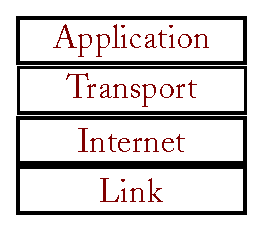
\includegraphics[width=5 cm]{layers.pdf}}\only<2>{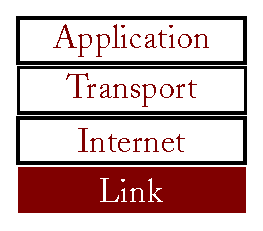
\includegraphics[width=5 cm]{link.pdf}}\only<3>{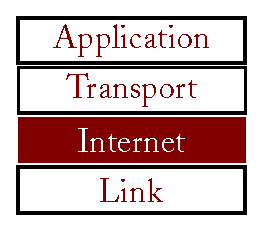
\includegraphics[width=5 cm]{internet.pdf}}\only<4>{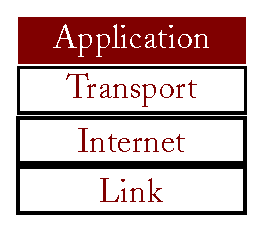
\includegraphics[width=5 cm]{application.pdf}}\only<5>{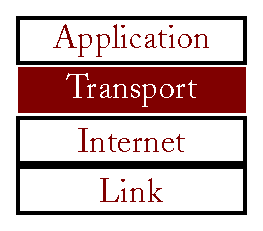
\includegraphics[width=5 cm]{transport.pdf}}

\end{column}

\begin{column}{0.5 \textwidth}

\begin{itemize}

\only<1>{
\item[]
}

\only<2>{
\item Wi-Fi

\item Cellular networks

\item Datacenters

\item 10 GigE

\item Transoceanic links
}

\only<3>{
\item Ubiquitous mobility
}

\only<4>{
\item Short flows (Web)

\item Streaming video (YouTube/Netflix)

\item Conferencing (Skype/Facetime)
}

\only<5>{
\item \colorbox{LightBlue}{{\LARGE \bf ???}}
}

\end{itemize}

\end{column}

\end{columns}

\end{frame}

\begin{frame}
\frametitle{Coping with change}

\Large

\mbox{\textcolor{DarkBlue}{How should protocols deal with an evolving network?}}

\vspace{\baselineskip}
\vspace{\baselineskip}

\textcolor{DarkGreen}{One approach: \textbf{design new protocols}.}

\end{frame}

\begin{frame}
\frametitle{The march of congestion-control protocols}
\only<1>{\noindent \hspace{-.75 cm} 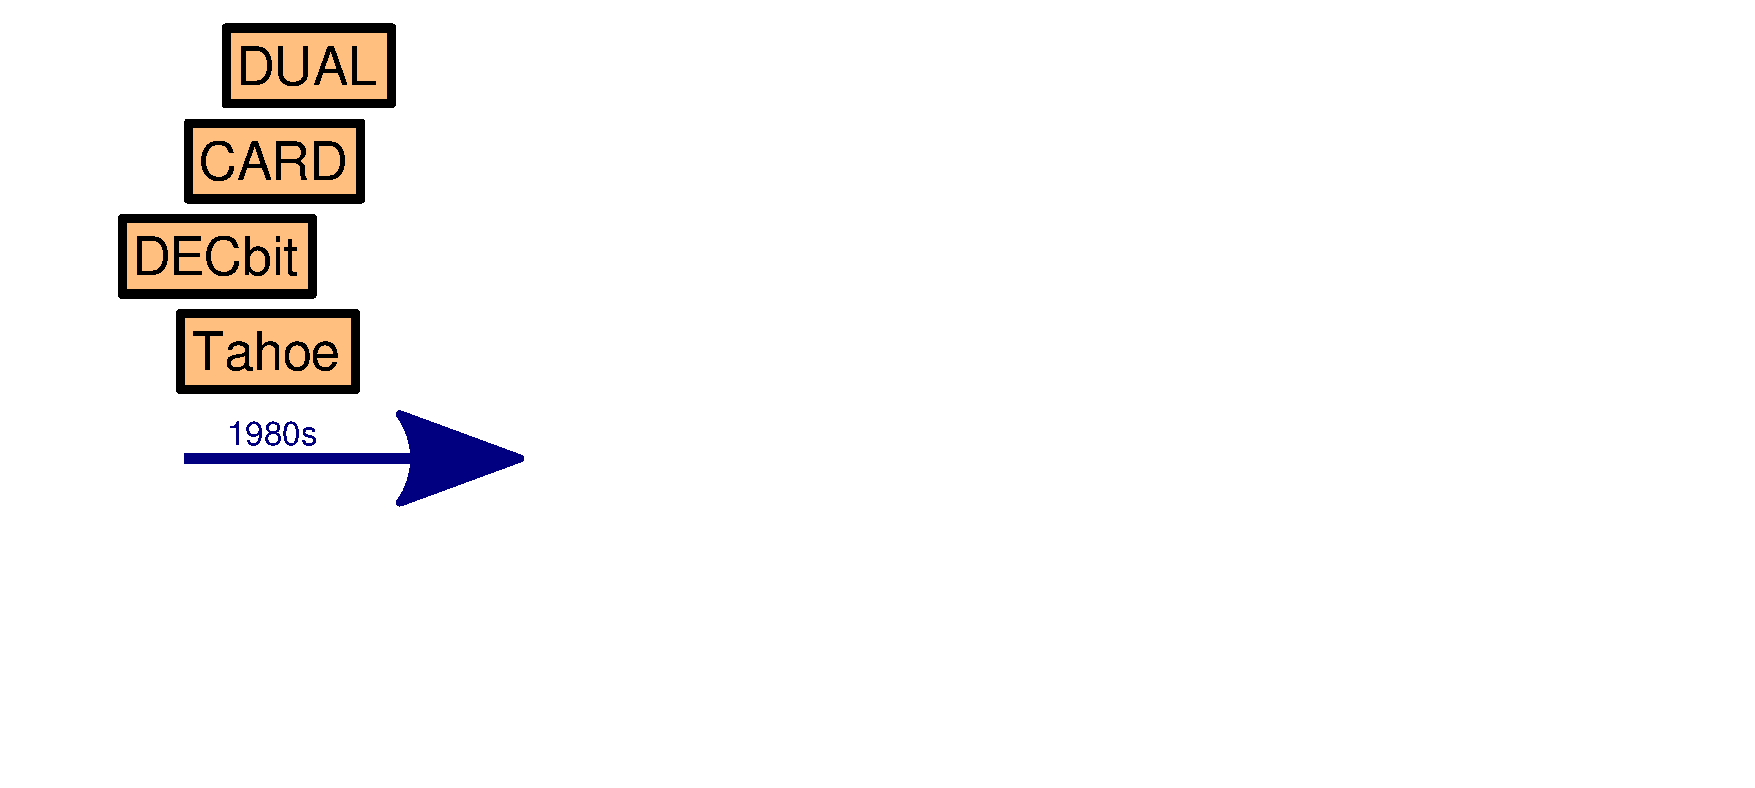
\includegraphics[width=1.1\textwidth]{march2-1.pdf}

}
\only<2>{\noindent \hspace{-.75 cm} 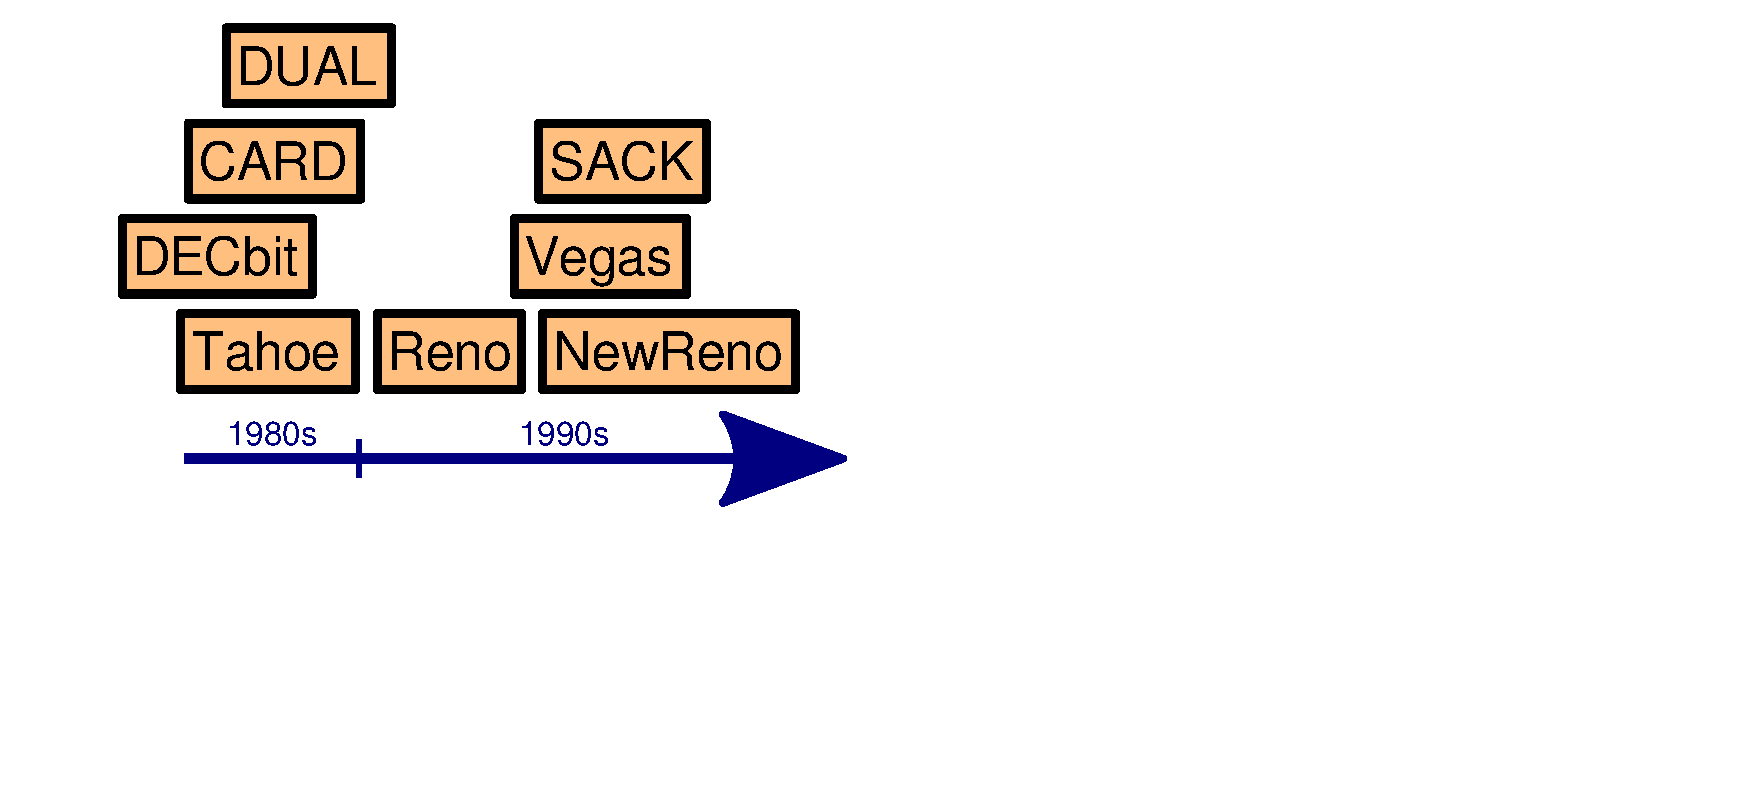
\includegraphics[width=1.1\textwidth]{march2-2.pdf}

}
\only<3>{\noindent \hspace{-.75 cm} 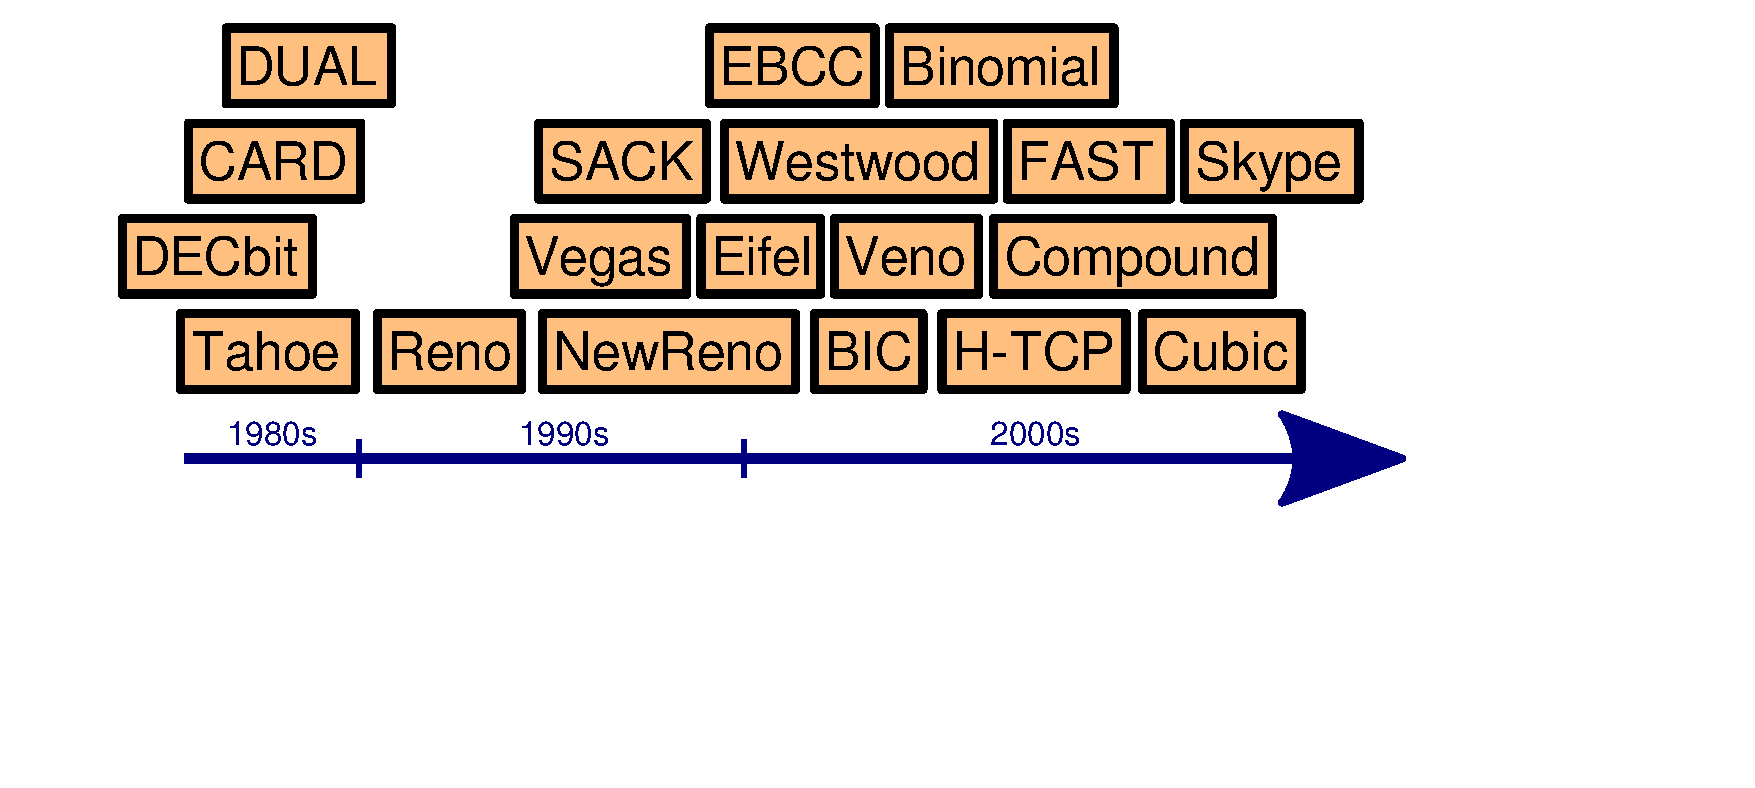
\includegraphics[width=1.1\textwidth]{march2-3.pdf}

}
\only<4>{\noindent \hspace{-.75 cm} 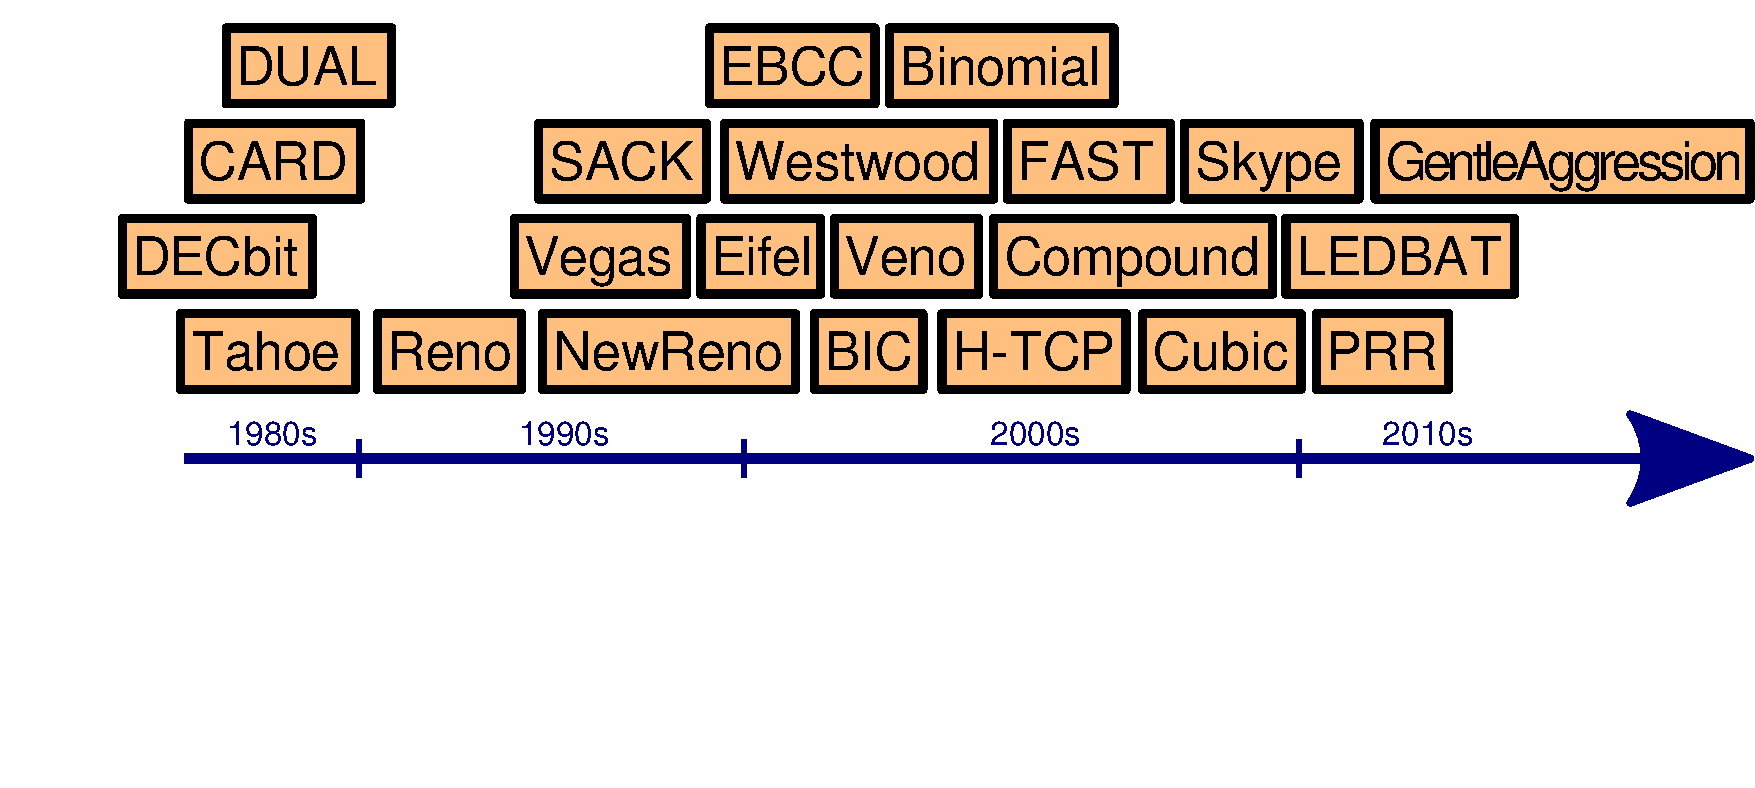
\includegraphics[width=1.1\textwidth]{march2-4.pdf}

}
\only<5>{\noindent \hspace{-.75 cm} 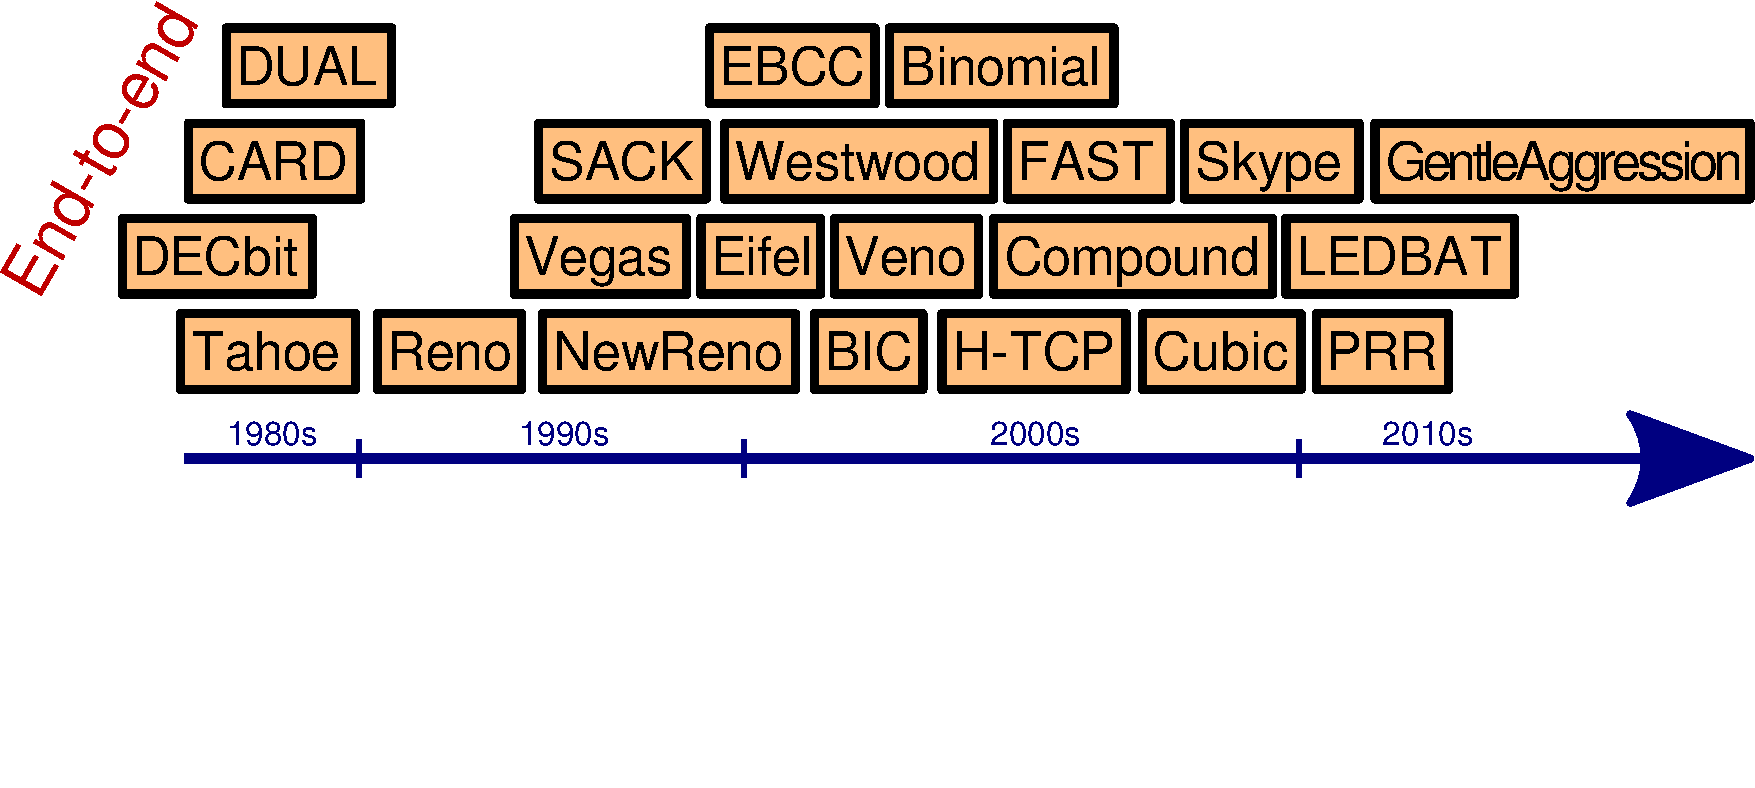
\includegraphics[width=1.1\textwidth]{march2-5b.pdf}

}
\only<6>{\noindent \hspace{-.75 cm} 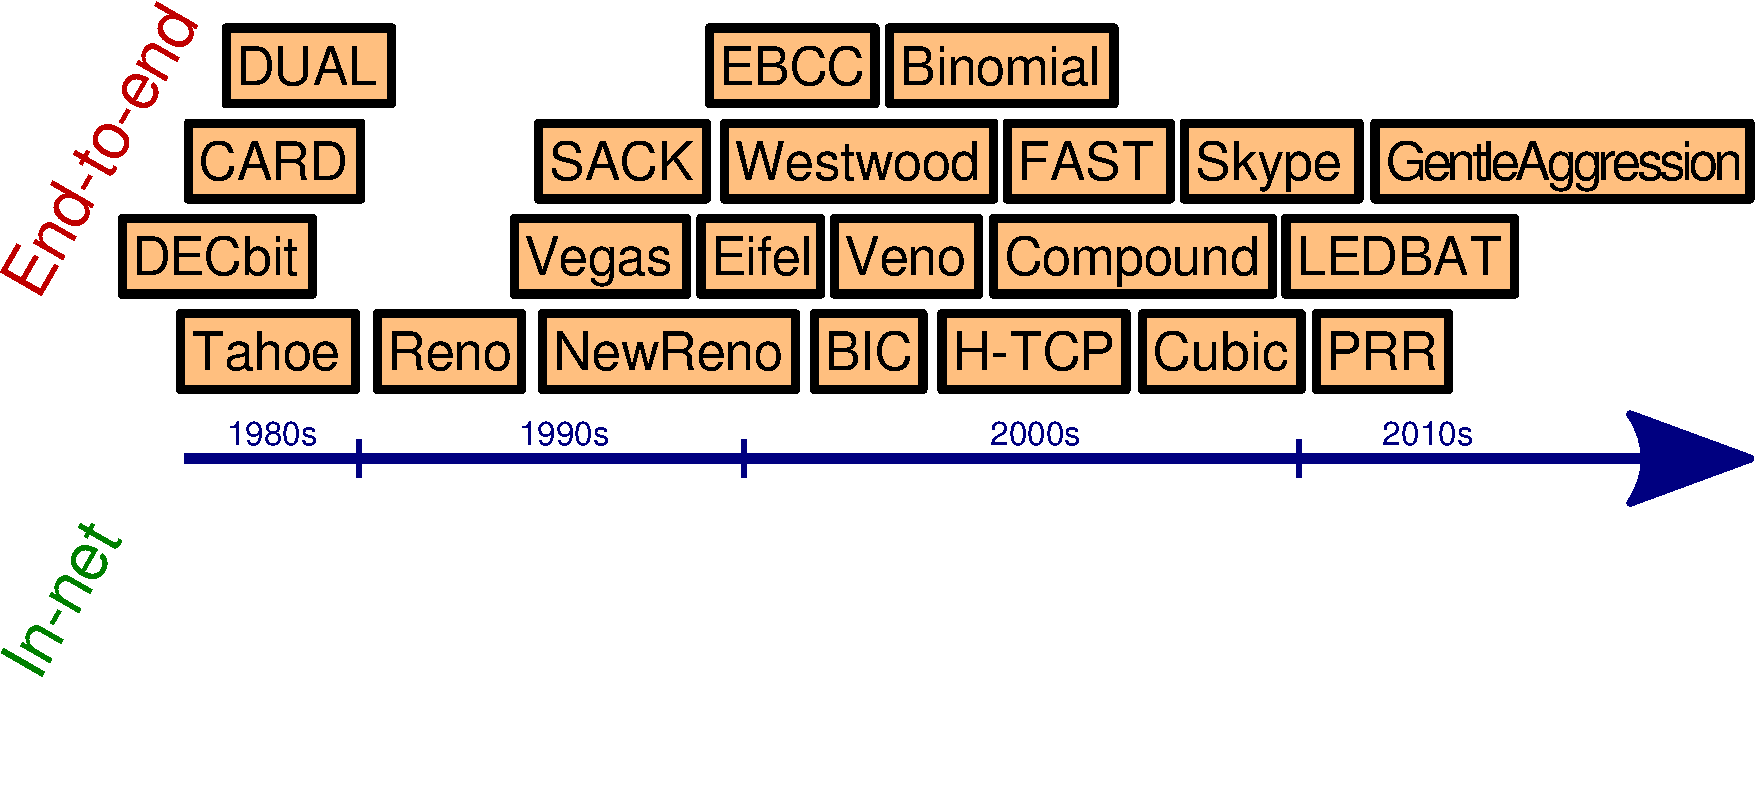
\includegraphics[width=1.1\textwidth]{march2-5.pdf}

}
\only<7>{\noindent \hspace{-.75 cm} 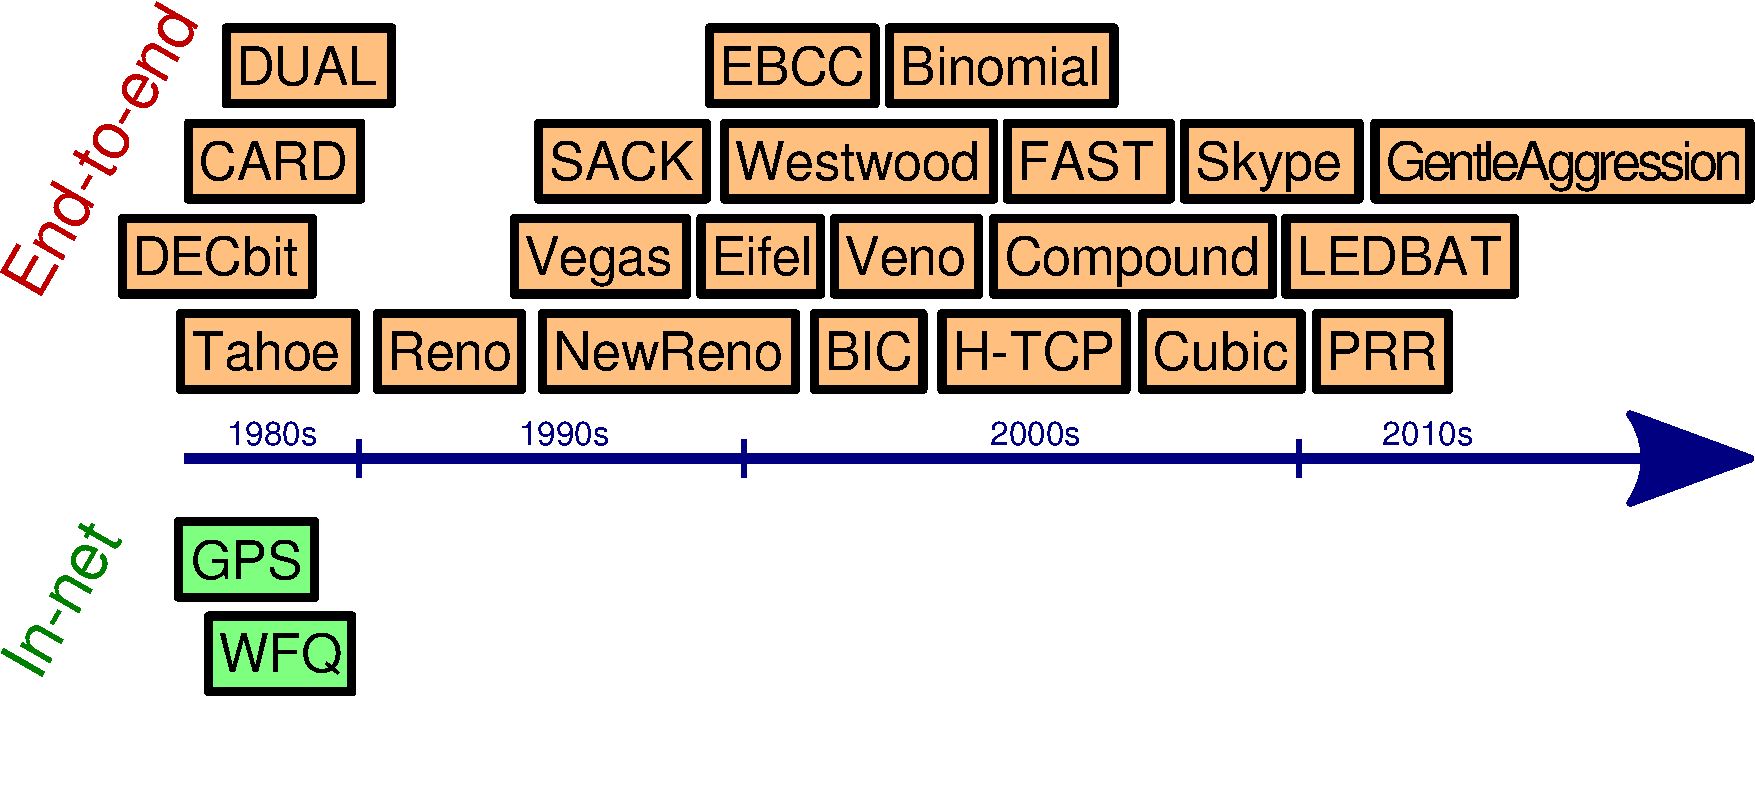
\includegraphics[width=1.1\textwidth]{march2-6.pdf}

}
\only<8>{\noindent \hspace{-.75 cm} 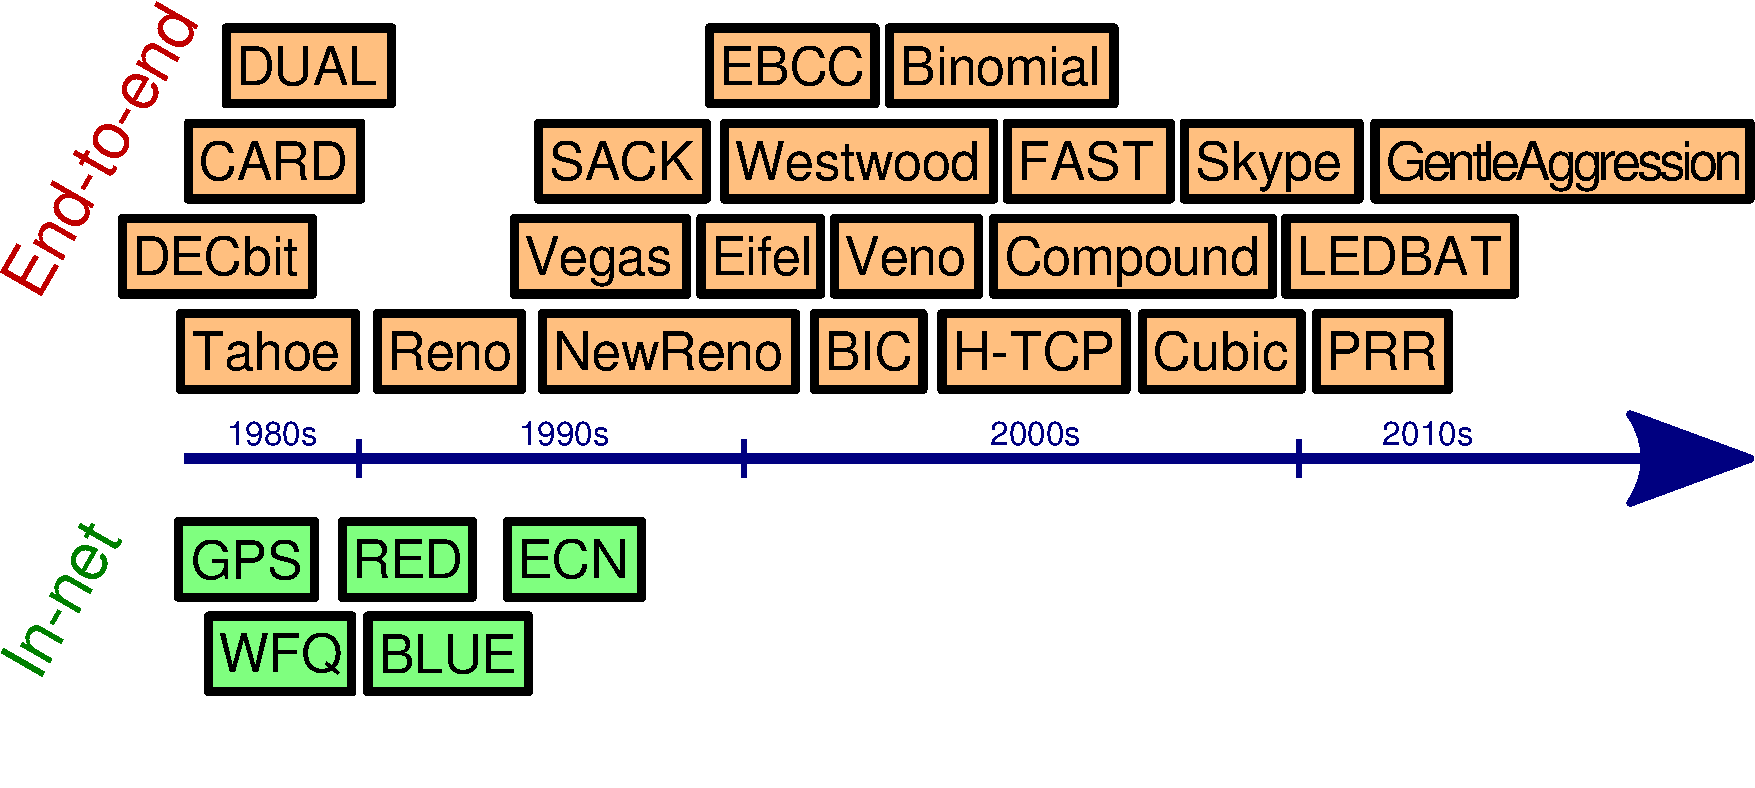
\includegraphics[width=1.1\textwidth]{march2-7.pdf}

}
\only<9>{\noindent \hspace{-.75 cm} 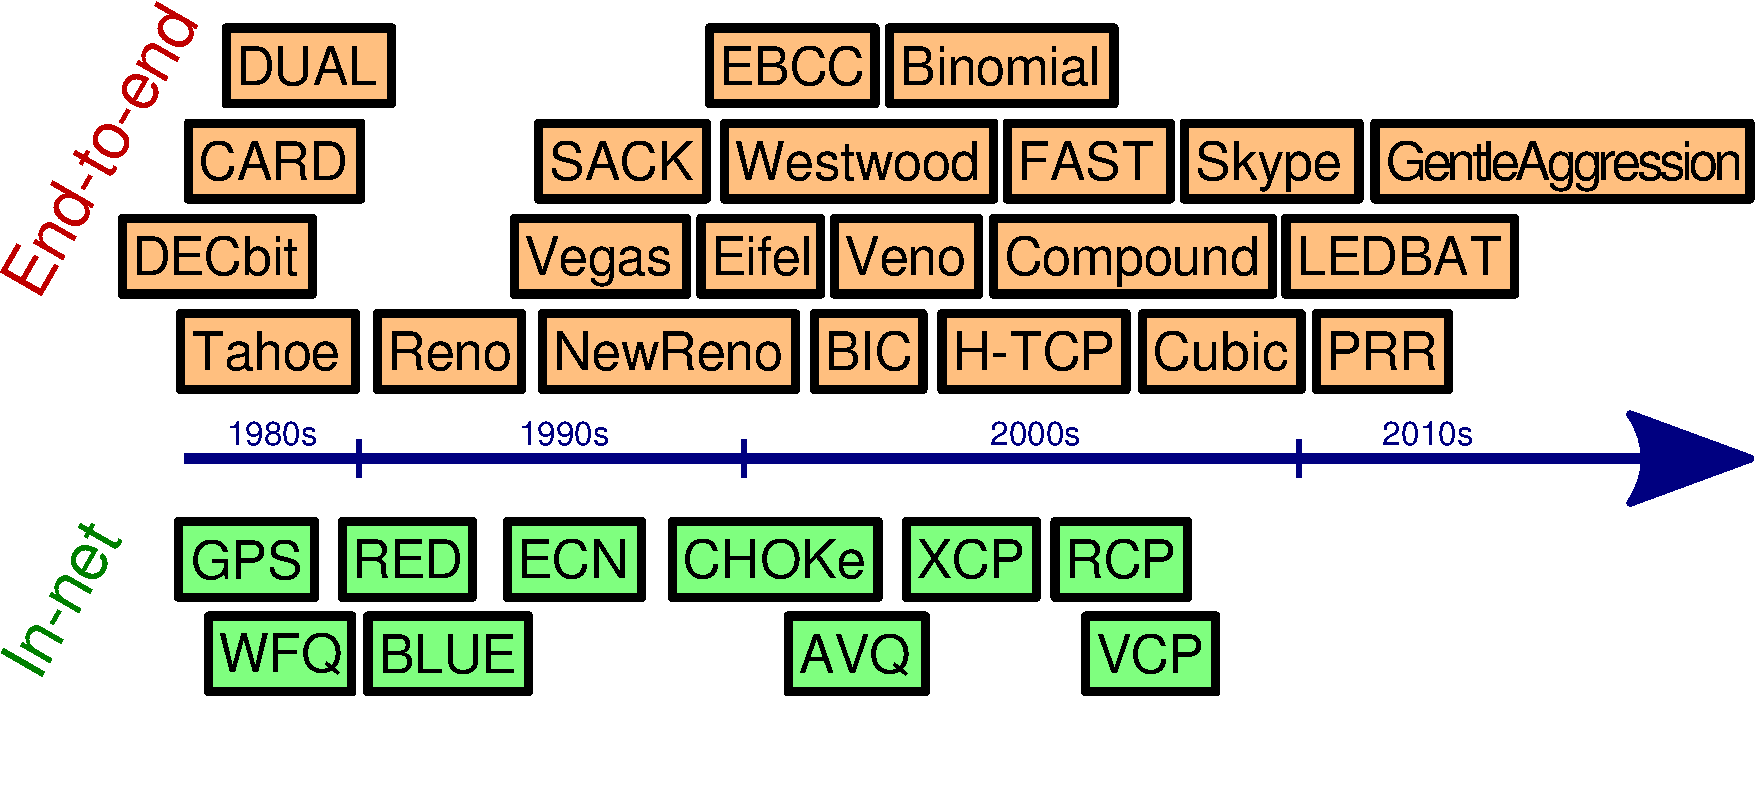
\includegraphics[width=1.1\textwidth]{march2-8.pdf}

}
\only<10>{\noindent \hspace{-.75 cm} 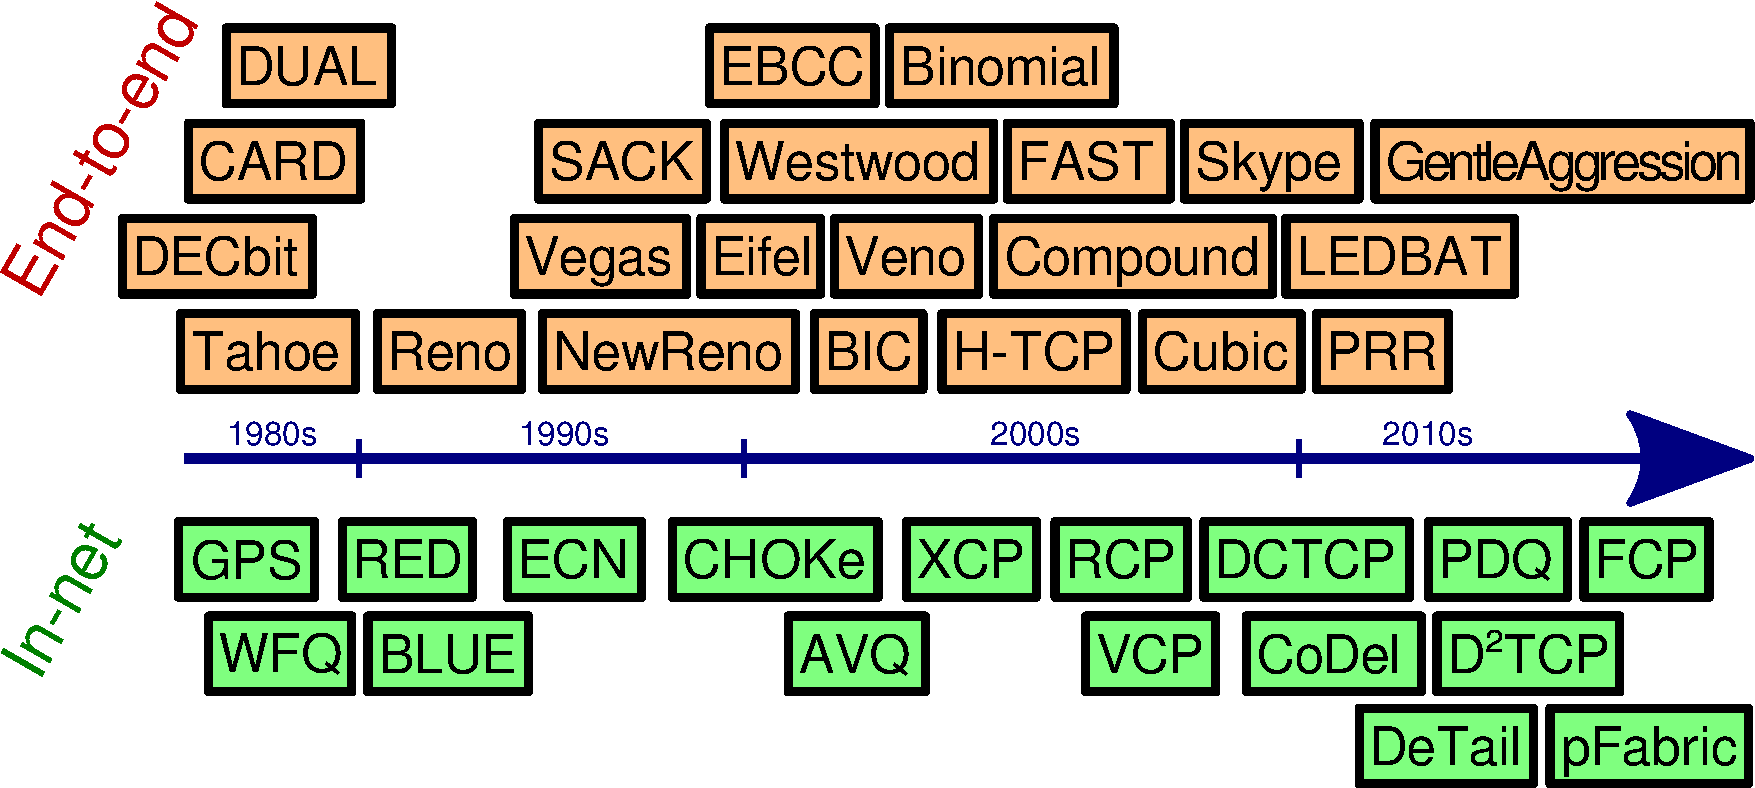
\includegraphics[width=1.1\textwidth]{march2-9.pdf}

}
\end{frame}

\begin{comment}

\begin{frame}
\frametitle{Now that we have 40+ algorithms\ldots}

\Large

\begin{itemize}

%\item Sprout for cellular networks?

\item Wireless-TCP for Wi-Fi?

\item Fast-TCP for long-distance links?

\item Datacenter-TCP for datacenters?

\item CoDel for cable modems?



\item \textcolor{DarkGreen}{\bf TBA-TCP for tomorrow's networks?}

\end{itemize}

\end{frame}

\end{comment}

\begin{frame}
\frametitle{Rational choice among transports is challenging}

\begin{centering}

\includegraphics[height=20 pt]{cubic.pdf}\hspace{8 pt}{\bf vs.}\hspace{8 pt}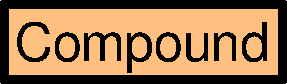
\includegraphics[height=20 pt]{compound.pdf}

\end{centering}

\ssline
\ssline
\ssline

\begin{itemize}

\Large

\item Different missions?

\item Different assumptions about network?

\item One scheme just plain better?

\end{itemize}

\end{frame}

\begin{frame}
\frametitle{Network evolution constrained by fuzzy assumptions}

\Large

On today's Internet:

\begin{columns}

\begin{column}{0.66\textwidth}

\begin{itemize}
\item Mask stochastic loss
\item[] \hspace{1 cm}$\rightarrow$ {\bf \textcolor{Maroon}{long delays}}
%\item Bufferbloat

\item No out-of-order delivery
\item[] \hspace{1 cm}$\rightarrow$ {\bf \textcolor{Maroon}{no parallel routing}}
\end{itemize}

\end{column}

\begin{column}{0.33\textwidth}

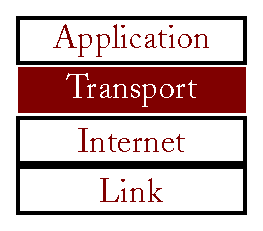
\includegraphics[width=\textwidth]{transport.pdf}

\end{column}

\end{columns}

\vspace{\baselineskip}

{\it Advice for Internet Subnetwork Designers}\\ (RFC 3819) is 21,000 words!

\end{frame}

\begin{comment}

\begin{frame}
\frametitle{Transport protocols}

\begin{centering}
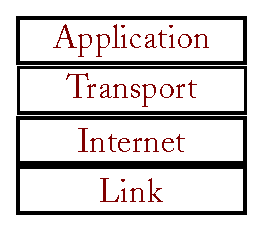
\includegraphics[width=8 cm]{layers.pdf}

\end{centering}

\end{frame}

\end{comment}

\begin{frame}
\frametitle{\textbf{Idea}: computer-generated transport}

\Large Transport layer should adapt to \textbf{whatever}

\begin{columns}

\begin{column}{0.66 \textwidth}

\begin{itemize}
\item network may do (\textbf{\textcolor{DarkBlue}{model}})

\item application wants (\textbf{\textcolor{DarkGreen}{mission}})

\end{itemize}

\end{column}

\begin{column}{0.33\textwidth}

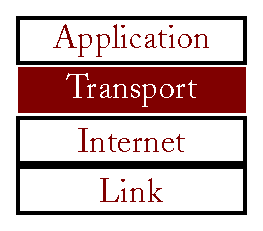
\includegraphics[width=\textwidth]{transport.pdf}

\end{column}

\end{columns}

\end{frame}

\begin{comment}

\begin{frame}
\frametitle{Our approach: declarative systems design}

\Large

\begin{centering}

\colorbox{Bisque}{
\begin{tabular}{l}
Computer-generated systems,\\
given a \textcolor{DarkBlue}{\bf model} and a \textcolor{DarkGreen}{\bf mission}.\\
\end{tabular}}


\end{centering}

\vspace{\baselineskip}
\vspace{\baselineskip}
\vspace{\baselineskip}

\noindent \textcolor{DarkBlue}{\bf model}: assumptions about the problem

\vspace{\baselineskip}

\textcolor{DarkGreen}{\bf mission}: objective that the users want

\end{frame}

\end{comment}

\begin{frame}
\frametitle{Contributions}

\begin{itemize}

\item[Sprout:] Protocol for interactive apps on cellular networks

\visible<2->{{\colorbox{Bisque}{\footnotesize\textbf{\textcolor{DarkBlue}{model}} = Cox process, \textbf{\textcolor{DarkGreen}{mission}} = max throughput with delay $<$ 0.1 s}}}

\item[]

\item[Remy:] Design tool that generates congestion-control algorithms

\visible<3->{{\colorbox{Bisque}{\footnotesize\textbf{\textcolor{DarkBlue}{model}} = user-specified networks \& workloads, \textbf{\textcolor{DarkGreen}{mission}} = user-specified}}}

\item[]

\end{itemize}

\hrule

\begin{itemize}

\item[]

\item[Mosh:] Mobile shell

\visible<4->{{\colorbox{Bisque}{\footnotesize\textbf{\textcolor{DarkBlue}{model}} = ANSI terminal, \textbf{\textcolor{DarkGreen}{mission}} = convey \textit{latest} frame}}}

\item[]

\item[Alfalfa:] Network video that optimizes an objective function

\visible<5->{{\colorbox{Bisque}{\footnotesize\textbf{\textcolor{DarkBlue}{model}} = varying net, \textbf{\textcolor{DarkGreen}{mission}} = quality vs.~startup vs.~stalls}}}

\end{itemize}

\end{frame}

\begin{frame}
\frametitle{Main takeaway}

\Large

In systems design, \textbf{\textcolor{DarkBlue}{showing our
    work}$^{*}$} yields better performance, and frees adjacent systems
to evolve.

\vspace{\baselineskip}
\vspace{\baselineskip}
\vspace{\baselineskip}

\normalsize

\textcolor{DarkBlue}{\textbf{*} (clearly enough for a computer to recreate the design)}

\end{frame}

\section{Sprout}

\begin{frame}
\frametitle{Sprout: a transport protocol designed for variability}

\large

\textit{\bf Observation:}

\hspace{10 pt} \colorbox{Bisque}{Videoconferences perform poorly over cellular networks.}

\vspace{\baselineskip}

\end{frame}

\begin{frame}
\frametitle{Verizon LTE throughput is highly variable}

\begin{centering}

{\small
\def\svgwidth{\columnwidth}\input{allcapacity.pdf_tex}
}

\end{centering}

\end{frame}

\begin{frame}
\frametitle{During a download, LTE delays packets for $>10$ seconds}

\begin{centering}

{\small
\def\svgwidth{0.8 \columnwidth}\input{pings.pdf_tex}
}

\end{centering}

\end{frame}

\begin{frame}
\frametitle{Interactive apps work poorly}

\begin{itemize}
\item We measured cellular networks while driving:

\begin{itemize}
\item {\color{red}\bf Verizon LTE}
\item Verizon 3G (1xEV-DO)
\item AT\&T LTE
\item T-Mobile 3G (UMTS)
\end{itemize}

\item Then ran apps across replayed network trace:

\begin{itemize}
\item {\color{red}\bf Skype} (Windows 7)
\item Google Hangouts (Chrome on Windows 7)
\item Apple Facetime (OS X)
\end{itemize}

\end{itemize}

\end{frame}

\begin{frame}
\frametitle{Skype's performance}

\end{frame}

\begin{frame}
\frametitle{Performance summary}

{
\def\svgwidth{\columnwidth}\footnotesize\import{dotgraphs3/}{VerizonLTE-Downlink-minus4.pdf_tex}
}
\end{frame}

\begin{frame}
\frametitle{What's wrong?}

\begin{itemize}
\item Existing schemes \textbf{react} to congestion signals.

\begin{itemize}
\item Packet loss.
\item Increase in round-trip time.
\end{itemize}

\item Feedback comes too late.

\item The killer: \textbf{self-inflicted queueing delay}.

\end{itemize}

\end{frame}

\begin{frame}
\frametitle{Question}

\begin{centering}
\colorbox{LightBlue}{
\begin{tabular}{p{4 in}}
\LARGE Can a transport protocol that's a function of
a \textbf{\textcolor{DarkBlue}{model}} and
\textbf{\textcolor{DarkGreen}{mission}} do better?
\end{tabular}}

\end{centering}

\end{frame}

\begin{frame}
\frametitle{Sprout's \textcolor{DarkGreen}{\bf mission}}

\Large

\begin{itemize}
\item Most throughput
\item Bounded risk of delay $>$ 100~ms
\end{itemize}

\vspace{\baselineskip}
\vspace{\baselineskip}
\vspace{\baselineskip}

\scriptsize

KW, Anirudh Sivaraman, and Hari Balakrishnan, \textbf{Stochastic Forecasts Achieve High Throughput and Low Delay over Cellular Networks}, \textit{USENIX NSDI 2013}

\end{frame}

\begin{frame}
\frametitle{Bounded risk of delay}
\begin{itemize}

\large

\item \textbf{Model} variation in link speed

\item \textbf{Infer} current link speed

\item \textbf{Predict} future link speed

\begin{itemize}
\item Don't wait for congestion
\end{itemize}

\item \textbf{Control:} Send as much as possible, but require:

\begin{itemize}

\item 95\% chance all packets arrive within 100~ms

\end{itemize}

\end{itemize}

\end{frame}

\begin{frame}
\frametitle{\textbf{Model}: packet deliveries looks like flicker noise}

\begin{centering}

\def\svgwidth{0.7 \columnwidth}\input{vz-inter.pdf_tex}

\end{centering}

{\small (Verizon LTE, phone stationary.)}

\end{frame}

\begin{frame}
\frametitle{\textbf{Model}: average rate looks like random walk}

\begin{centering}

{\small
\def\svgwidth{\columnwidth}\input{allcapacity.pdf_tex}
}

\end{centering}

\end{frame}

\begin{frame}

\begin{centering}
\frametitle{Sprout's \textcolor{DarkBlue}{\bf model}: G/M/1 queue}
\def\svgwidth{\columnwidth}\input{sprout-model.pdf_tex}

\end{centering}

%\vspace{\baselineskip}

%All source code was \bf{\textcolor{DarkGreen}{frozen before data collection began.}}

\end{frame}

\begin{comment}

\begin{frame}
\frametitle{Sprout's model parameters}

\begin{tabular}{ll}
Volatility $\sigma$: fixed @ & $200~\frac{\textrm{pkts}/s}{\sqrt{s}}$ \\

Expected outage time $1/\lambda_z$: & $1~s$ \\

Tick length ($\tau$): & $20~ms$ \\

Forecast length: & $160~ms$ \\

Delay target: & $100~ms$ \\

Risk tolerance: & $5 \%$ \\
\end{tabular}

\vspace{\baselineskip}

All source code was \bf{\textcolor{DarkGreen}{frozen before data collection began.}}

\end{frame}

\end{comment}

\begin{frame}
\frametitle{\textbf{Infer}: current link speed}

\Large

\begin{itemize}

\item \textcolor{DarkBlue}{\bf Observe} packets received every $\tau$

\item[]

\item \textcolor{DarkGreen}{\bf Update} P($\lambda$)

\end{itemize}

\end{frame}

\begin{frame}
\frametitle{\textbf{Predict}: future link speed}

\Large

\begin{itemize}
\item \textcolor{DarkBlue}{\bf Evolve} model forward

\item[]

\item \textcolor{DarkGreen}{\bf Forecast} 5th percentile cumulative packets

%\item Almost all precalculated

\end{itemize}

\end{frame}

\begin{frame}
\frametitle{\textbf{Control}: fill up 100~ms forecast window}
\begin{centering}
\only<1>{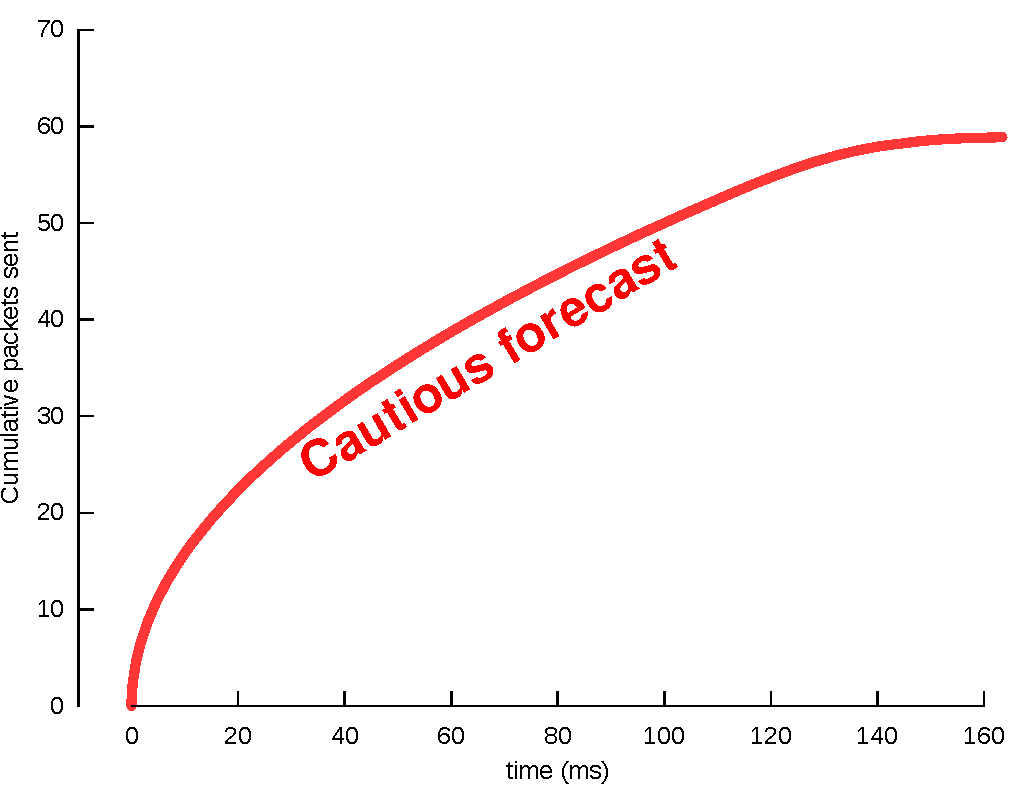
\includegraphics[width=0.9\columnwidth]{forecast-minus6.pdf}}\only<2>{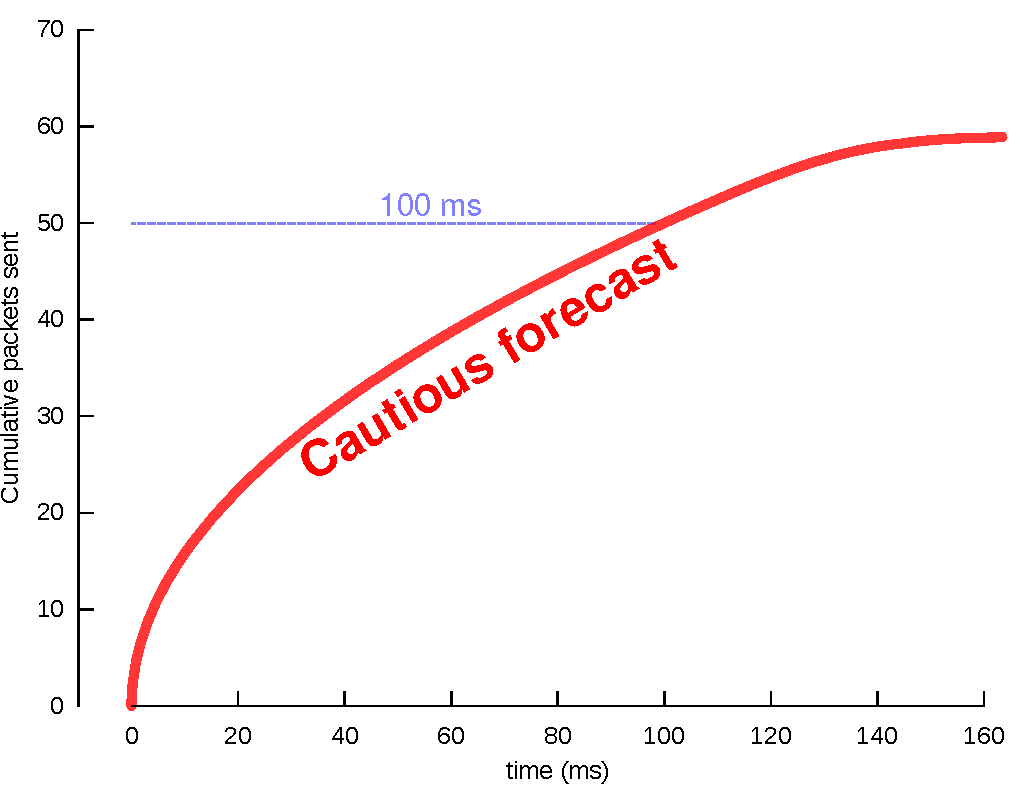
\includegraphics[width=0.9\columnwidth]{forecast-minus5.pdf}}\only<3>{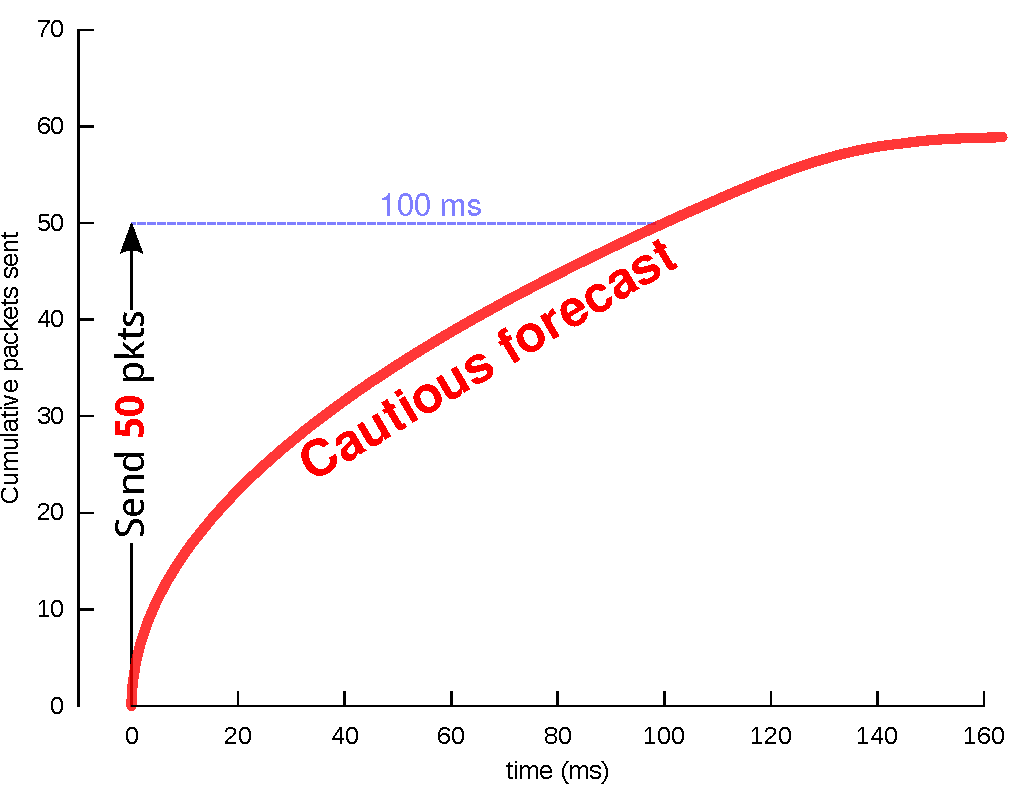
\includegraphics[width=0.9\columnwidth]{forecast-minus4.pdf}}\only<4>{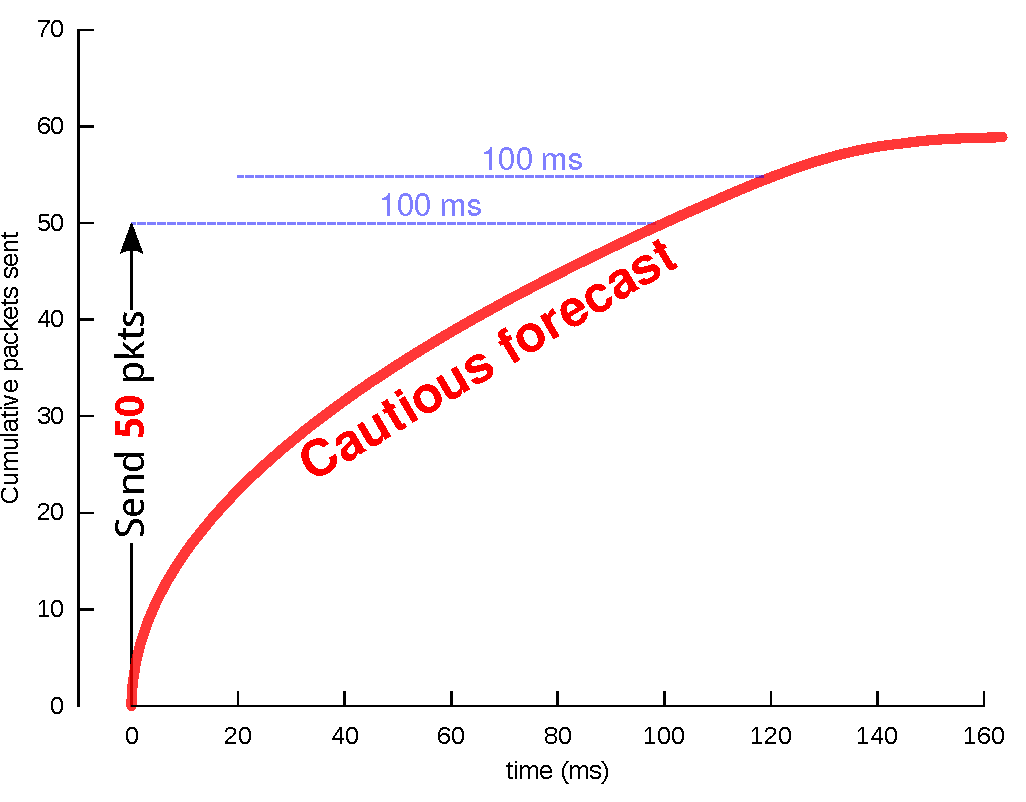
\includegraphics[width=0.9\columnwidth]{forecast-minus3.pdf}}\only<5>{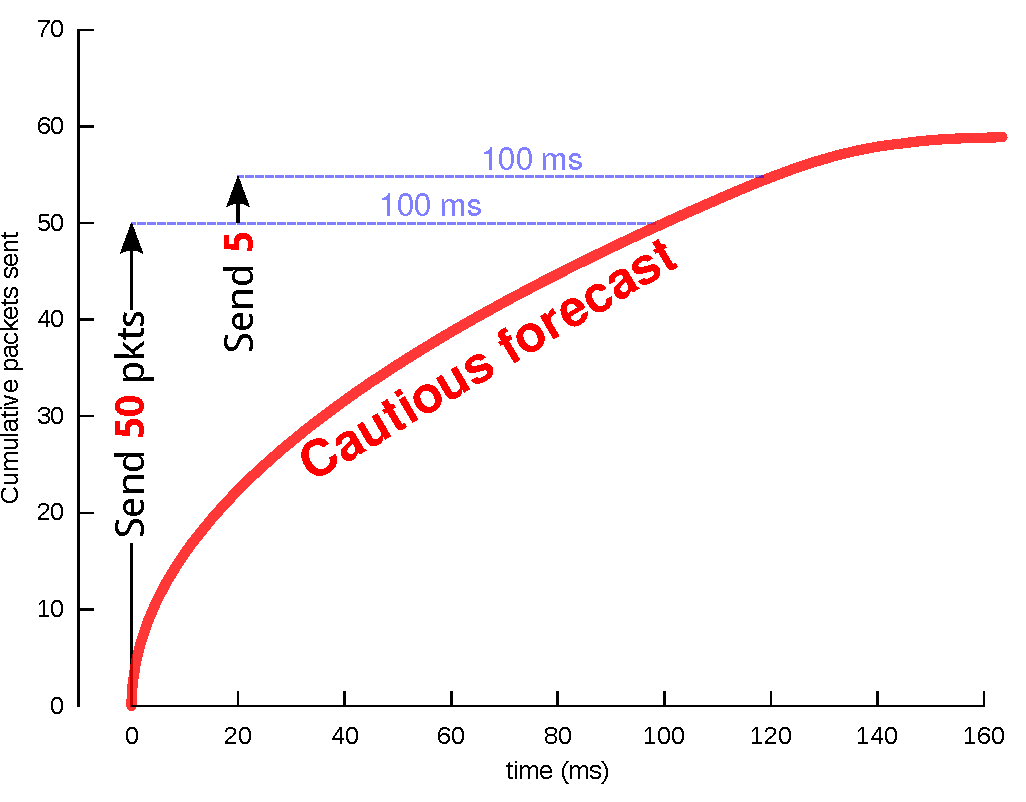
\includegraphics[width=0.9\columnwidth]{forecast-minus2.pdf}}\only<6>{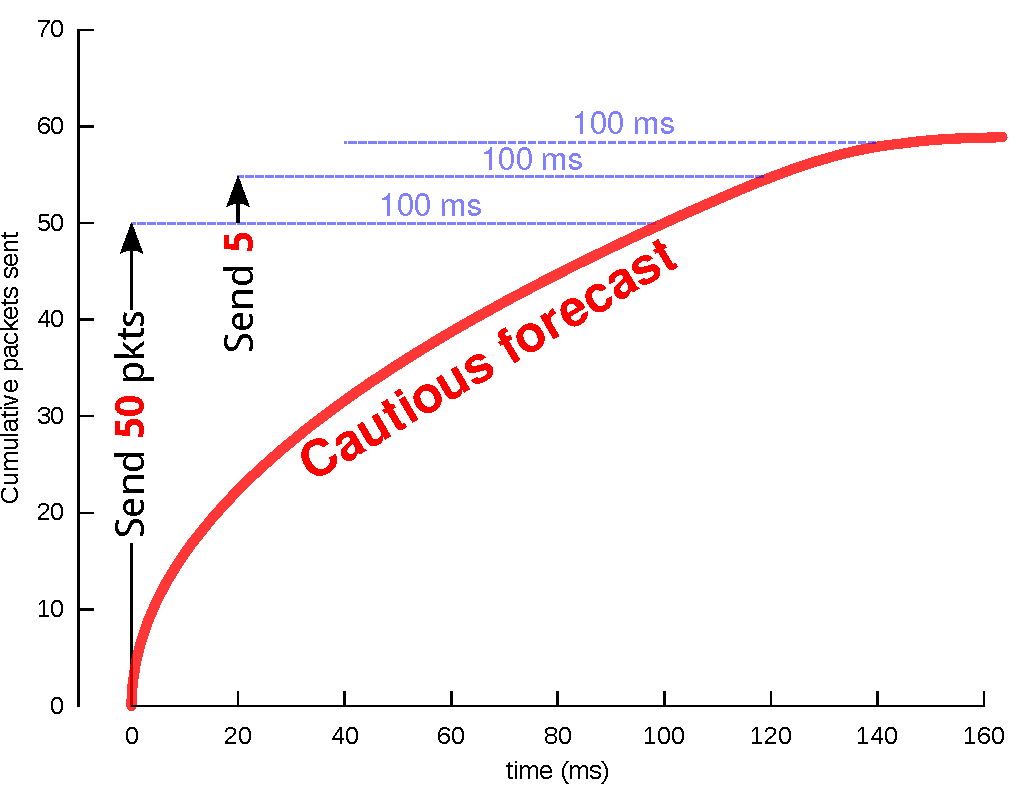
\includegraphics[width=0.9\columnwidth]{forecast-minus1.pdf}}\only<7>{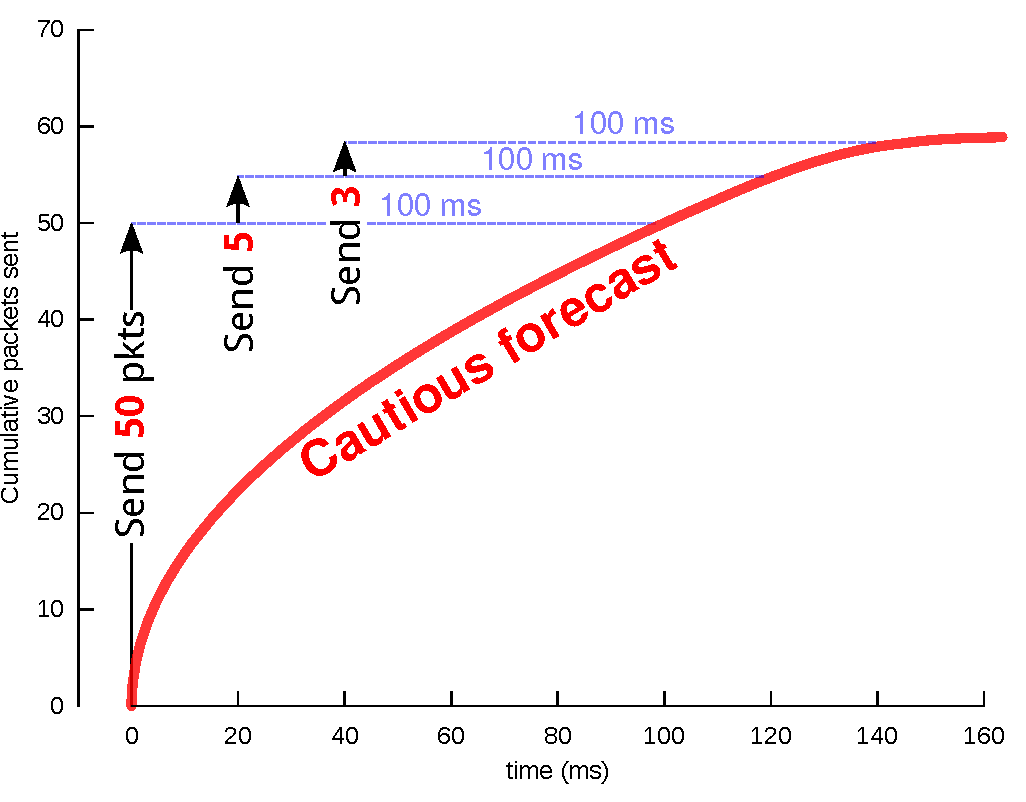
\includegraphics[width=0.9\columnwidth]{forecast-final.pdf}}

\end{centering}
\end{frame}

\begin{frame}
\frametitle{Sprout's results}

\end{frame}

\begin{frame}
\only<1>{\def\svgwidth{\columnwidth}\footnotesize\import{dotgraphs3/}{VerizonLTE-Downlink-minus4.pdf_tex}}\only<2>{\def\svgwidth{\columnwidth}\footnotesize\import{dotgraphs3/}{VerizonLTE-Downlink-minus3.pdf_tex}}\only<3>{\def\svgwidth{\columnwidth}\footnotesize\import{dotgraphs3/}{VerizonLTE-Downlink-minus2.pdf_tex}}\only<4>{\def\svgwidth{\columnwidth}\footnotesize\import{dotgraphs3/}{VerizonLTE-Downlink-minus1.pdf_tex}}\only<5>{\def\svgwidth{\columnwidth}\footnotesize\import{dotgraphs3/}{VerizonLTE-Uplink.pdf_tex}}%\only<7>{\def\svgwidth{\columnwidth}\footnotesize\import{dotgraphs3/}{Verizon3G1xEV-DO-Downlink.pdf_tex}}\only<8>{\def\svgwidth{\columnwidth}\footnotesize\import{dotgraphs3/}{Verizon3G1xEV-DO-Uplink.pdf_tex}}\only<9>{\def\svgwidth{\columnwidth}\footnotesize\import{dotgraphs3/}{ATTLTE-Downlink.pdf_tex}}\only<10>{\def\svgwidth{\columnwidth}\footnotesize\import{dotgraphs3/}{ATTLTE-Uplink.pdf_tex}}\only<11>{\def\svgwidth{\columnwidth}\footnotesize\import{dotgraphs3/}{T-Mobile3GUMTS-Downlink.pdf_tex}}\only<12>{\def\svgwidth{\columnwidth}\footnotesize\import{dotgraphs3/}{T-Mobile3GUMTS-Uplink.pdf_tex}}
\end{frame}

\begin{frame}
\frametitle{Overall results on 8 links}

Verizon 3G/LTE, AT\&T LTE, T-Mobile 3G uplink and downlink:

\vspace{\baselineskip}

\begin{tabular}{|l|c|c|}
\hline
{\color{blue}Sprout} vs.~ & Avg.~speedup & Delay reduction \\
\hline
\hline
{\color{red}Skype} & $2.2\times$ & $7.9\times$ \\
{\color{red}Hangout} & $4.4\times$ & $7.2\times$ \\
{\color{red}Facetime} & $1.9\times$ & $8.7\times$ \\
\hline
{\color{ForestGreen}Compound} & $1.3\times$ & $4.8\times$ \\
{\color{ForestGreen}TCP Vegas} & $1.1\times$ & $2.1\times$ \\
{\color{ForestGreen}LEDBAT} & Same & $2.8\times$ \\
{\color{Orange}Cubic} & \cellcolor{red!20} $0.91\times$ & $79\times$ \\
%CUBIC/CoDel & & \\
%Compound/CoDel & & \\
\hline
\end{tabular}

\end{frame}

\begin{frame}
\frametitle{Sprout is end-to-end, but comparable to in-net control}
\vspace{-1 cm}
\def\svgwidth{\columnwidth}\footnotesize\import{dotgraphs3/}{Codels.pdf_tex}
\end{frame}

%\begin{frame}
%\frametitle{Replication by Stanford students (February--March 2013)}
%
%\large
%
%\begin{itemize}
%\item Alterman \& Quach reproduced part of Sprout paper
%
%\item[]
%
%\item {\scriptsize\texttt{http://ReproducingNetworkResearch.wordpress.com/2013/03/12/1216/}}
%
%\item[]
%
%\item Won best project award in Stanford networking class
%
%\end{itemize}
%
%\end{frame}

\begin{frame}
\frametitle{Question}

\begin{centering}
\colorbox{LightBlue}{
\LARGE Can a protocol do even better?}

\end{centering}

\end{frame}

\begin{frame}
\frametitle{M.I.T.~6.829 contest (March--April 2013)}

\begin{itemize}
\item Turnkey network emulator, evaluation

\item Sender, receiver run in Linux containers

\item \textbf{\textcolor{DarkGreen}{Mission}}: maximize throughput/delay

\item 4th prize: \$20

\item 3rd prize: \$30

\item 2nd prize: \$40

\item (If beat Sprout) 1st prize: \pause {\color{DarkBlue}{\bf Co-authorship on future paper}}

\end{itemize}

\vspace{\baselineskip}
\vspace{\baselineskip}
\vspace{\baselineskip}

\visible<3>{\scriptsize Anirudh Sivaraman, KW, Pauline Varley, Somak
  Das, Joshua Ma, Ameesh Goyal, Jo\~{a}o Batalha, and Hari Balakrishnan,
  \textbf{Protocol Design Contests}, \textit{in submission}}

\end{frame}

\begin{frame}
\frametitle{Baseline}

\begin{centering}
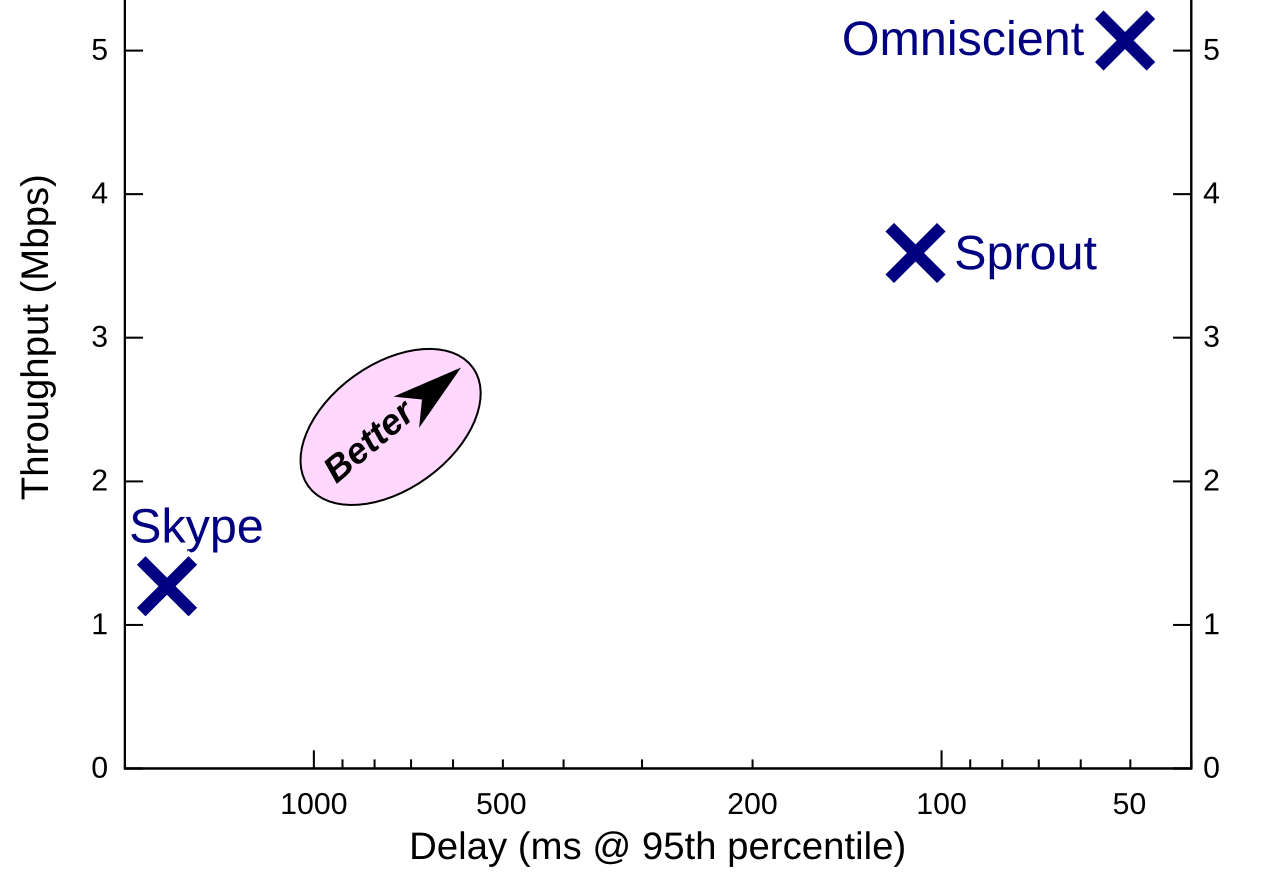
\includegraphics[width=0.9\columnwidth]{pointplot-nostudents.png}

\end{centering}

\end{frame}

\begin{frame}
\frametitle{Land of 3,000 student protocols}

\begin{centering}
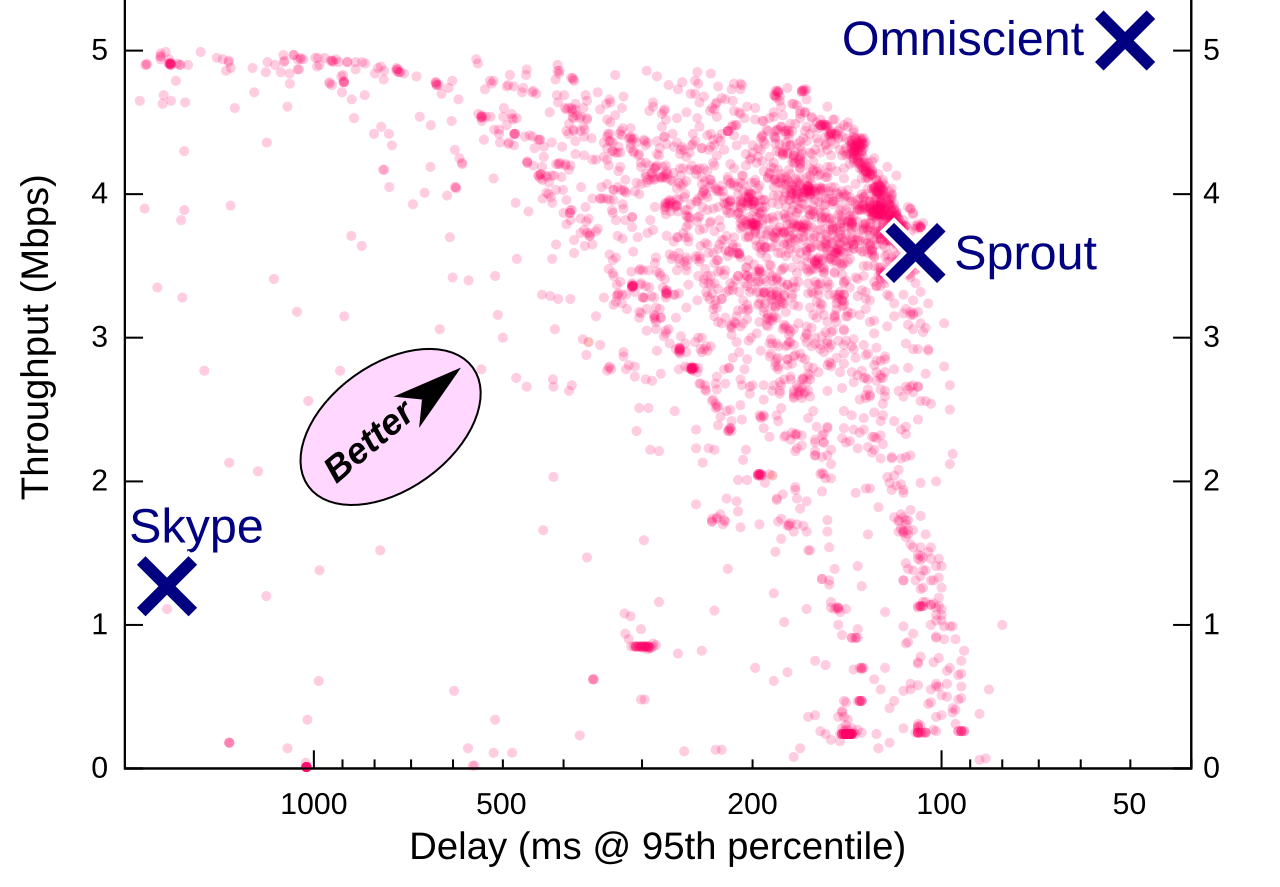
\includegraphics[width=0.9\columnwidth]{pointplot.png}

\end{centering}

\end{frame}

\begin{frame}
\frametitle{Sprout was on the frontier}

\begin{centering}
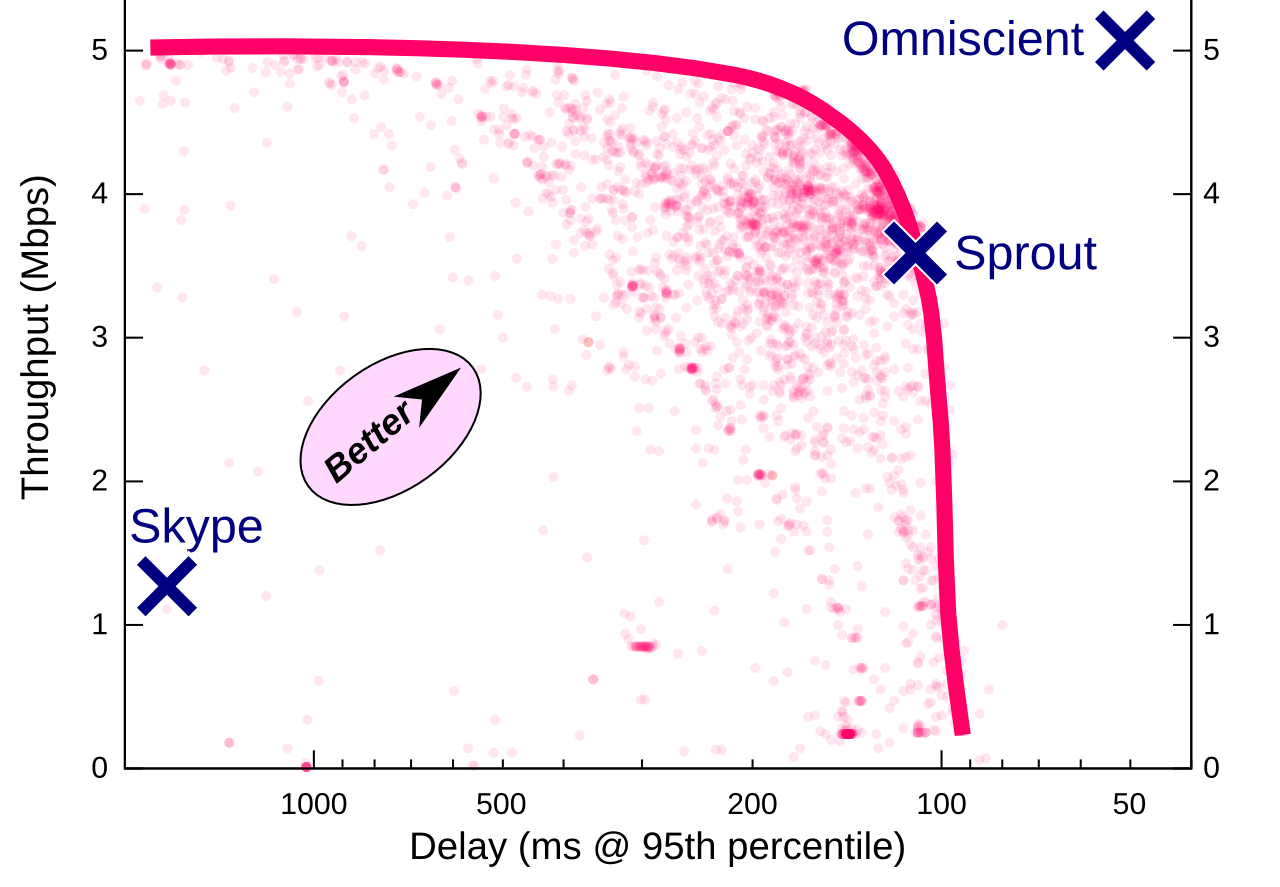
\includegraphics[width=0.9\columnwidth]{pointplot-withhull.png}

\end{centering}

\end{frame}

\begin{frame}
\frametitle{Commercial interest and implementations}

\begin{tabular}{cp{2 cm}c}


\includegraphics[width=4 cm]{screenhero.png} & & 
\includegraphics[width=4 cm]{highfive.png} \\

\\

\raisebox{0.8 ex}{
\includegraphics[width=3 cm]{Google_Logo_Old.PNG}} & 
\includegraphics[width=2.5 cm]{skype-logo.jpg} & \raisebox{-0.3cm}{
\includegraphics[width=2.5 cm]{viber.png}} \\

\\


\includegraphics[width=2.3 cm]{adobe-logo.jpg} & \raisebox{0.3 cm}{
\includegraphics[width=6 cm]{facebook-logo-face.jpeg}} \\

\end{tabular}

\end{frame}

\begin{frame}
\frametitle{Sprout's mark}

\only<1>{\noindent \hspace{-.75 cm} 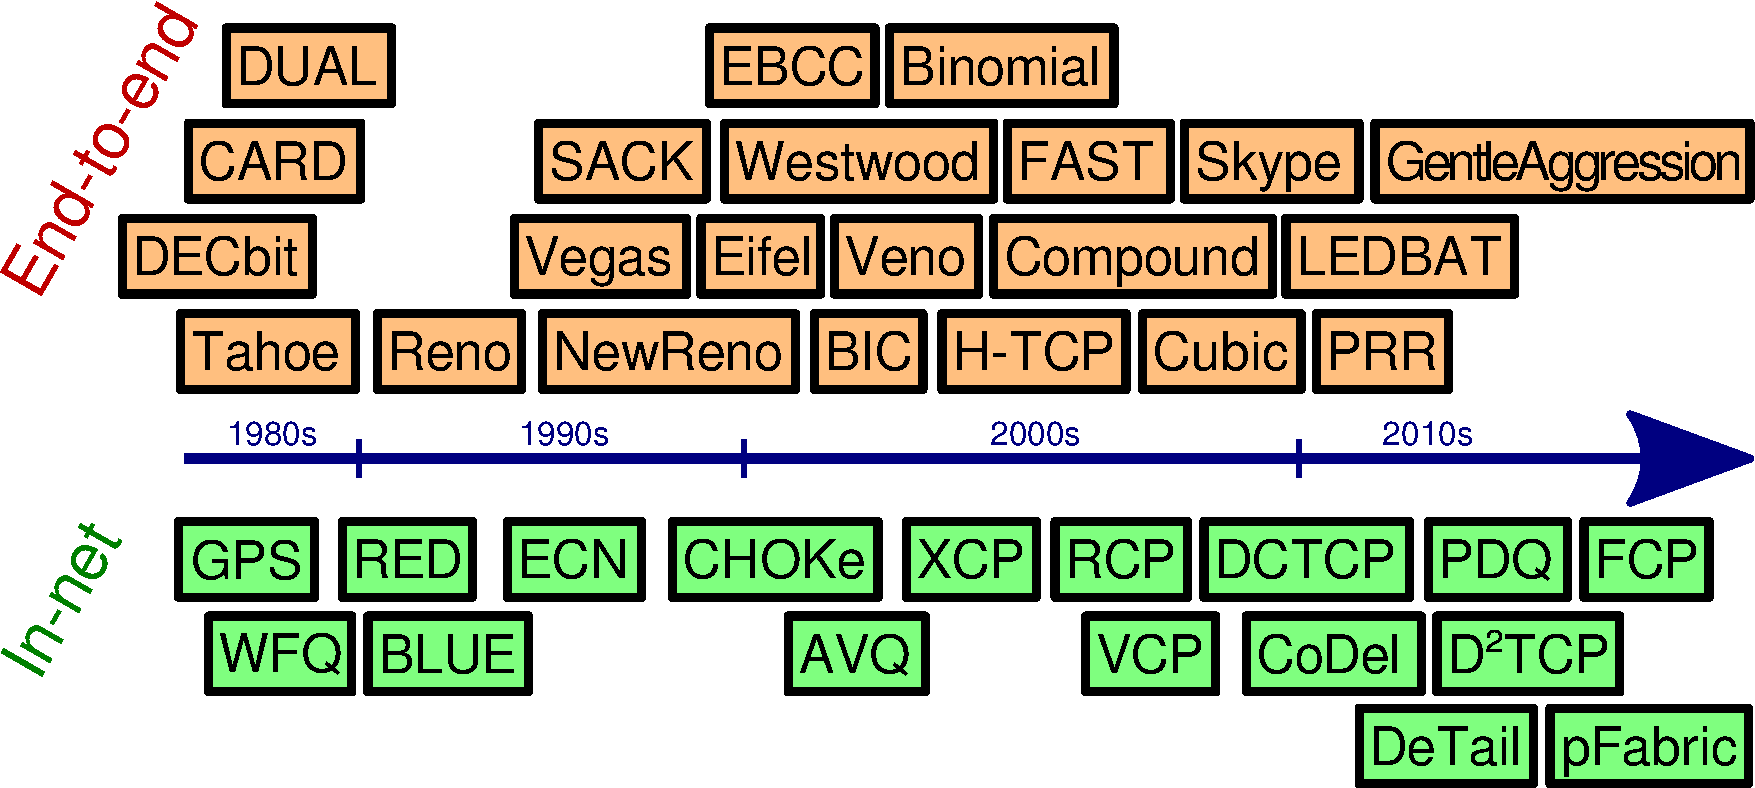
\includegraphics[width=1.1\textwidth]{march2-9.pdf}

}
\only<2>{\noindent \hspace{-.75 cm} 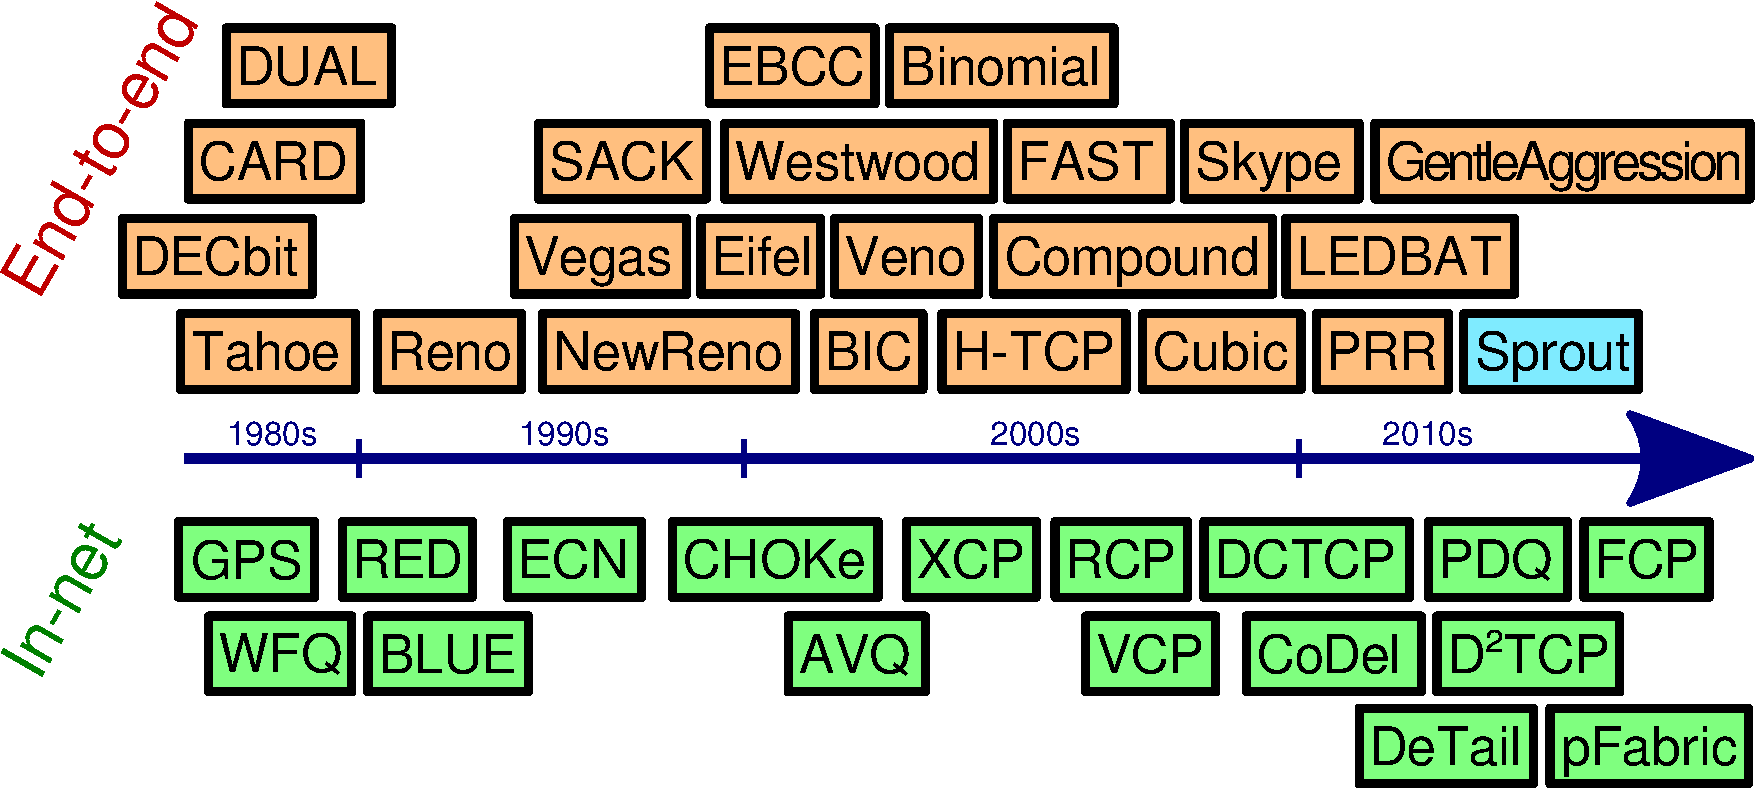
\includegraphics[width=1.1\textwidth]{march2-all.pdf}

}

\end{frame}

\begin{frame}

\only<1>{\frametitle{Cellular networks generally have {\bf per-user} queues}}
\only<2>{\frametitle{\ldots but Internet in general doesn't.}}
\only<3>{\frametitle{How can multiple contending users manage congestion?}}

\only<1>{\noindent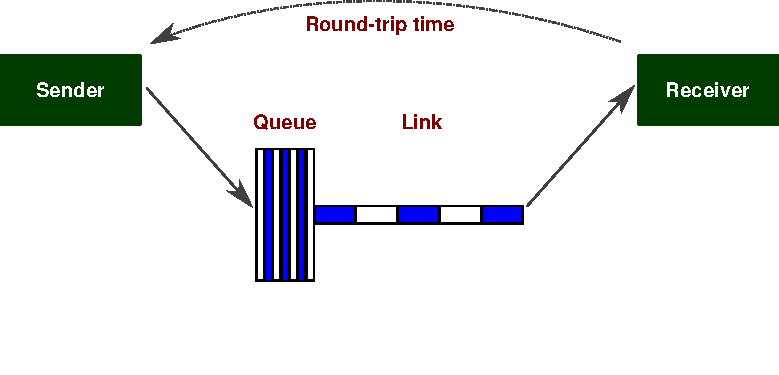
\includegraphics[width=\textwidth]{dumbbell-2.pdf}}\only<2>{\noindent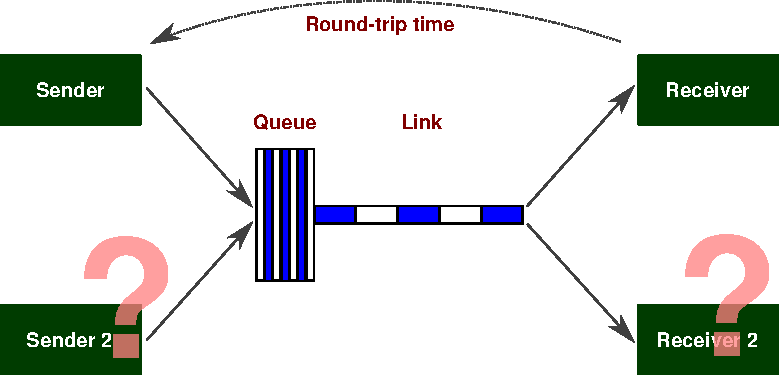
\includegraphics[width=\textwidth]{dumbbell-1.pdf}}\only<3>{\noindent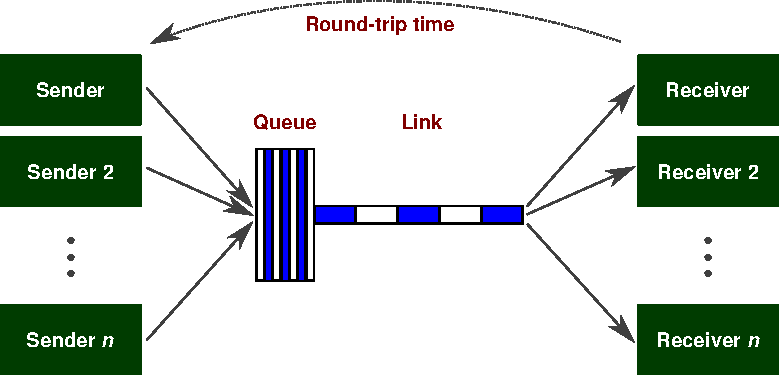
\includegraphics[width=\textwidth]{dumbbell.pdf}}

\end{frame}

\begin{comment}

\begin{frame}
\frametitle{Limitations of Sprout}

\Large

\begin{itemize}

\item Cells generally have \textcolor{DarkBlue}{\textbf{per-user}} queues\ldots

\item[] \ldots but Wi-Fi and wired networks usually don't.

\item[]

\item How to design for multiple contending users?

\end{itemize}

%\item[]

%\item Assumption: application always has data to send


\end{frame}

\end{comment}

\begin{comment}

\section{Remy}

\begin{frame}
\frametitle{Apps hack around TCP}

\Large

\begin{itemize}
\item Open lots of flows \hspace{1.9 cm} \only<2->{
\includegraphics[width=0.5cm]{firefox.png} \hspace{0.001 cm} 
\includegraphics[width=0.5cm]{chrome-64.png} \hspace{0.001 cm} 
\includegraphics[width=0.5cm]{Internet_Explorer_10_logo.png} \hspace{0.02 cm} 
\includegraphics[width=0.5cm]{safari.jpg} \hspace{0.02 cm} 
\includegraphics[width=0.5cm]{mozilladino.png}}

\item Goose slow start \only<3->{\hspace{2.18 cm} \raisebox{-0.6ex}{
\includegraphics[height=14 pt]{Google_Logo_Old.PNG}} \raisebox{-.125 ex}{
\includegraphics[height=10 pt]{mslogo.png}}}

\item Add pacing \hspace{3.3 cm} \only<4->{\raisebox{-.4 ex}{\includegraphics[height=14 pt]{youtube.png}}}

\item Give up and do it yourself

\visible<5>{
\small
\hspace{5.95 cm}\begin{minipage}{3.5 cm}
{\bf Chrome} \textcolor{DarkBlue}{(QUIC)} \\
{\bf BitTorrent} \textcolor{DarkBlue}{($\mu$TP)} \\
{\bf Mosh} \textcolor{DarkBlue}{(SSP)} \\
{\bf IBM Aspera} \textcolor{DarkBlue}{(fasp)} \\
\end{minipage}
}

\end{itemize}

\end{frame}

\end{comment}

\begin{frame}
\frametitle{Question}

\begin{centering}
\colorbox{LightBlue}{
\begin{tabular}{p{4.2 in}}
\LARGE Can a computer-generated transport \mbox{protocol}
solve \textbf{multi-user} congestion control?
\end{tabular}}

\end{centering}

\end{frame}

\begin{frame}
\frametitle{Prior work (abridged)}

\begin{itemize}

\item {\bf \textcolor{DarkBlue}{Jacobson (1988):}} additive-increase, multiplicative-decrease

\item[]

\item {\bf \textcolor{DarkBlue}{Kelly, Maulloo \& Tan (1998):}} optimization problem that AIMD solves {\it asymptotically}

\item[]

\item {\bf \textcolor{DarkBlue}{Yi \& Chiang (2008):}} stochastic network utility maximization

\end{itemize}

\end{frame}

\begin{frame}
\only<1>{\frametitle{The basic question of distributed congestion control}}
\only<2>{\frametitle{Super\textcolor{Black}{rat}ional congestion control}}

\begin{centering}
\fbox{
\begin{minipage}{6 cm}
\LARGE At this moment,\visible<1->{\textcolor{DarkBlue}{\bf *}} do I:

\begin{itemize}

\item send a packet
\item not send a packet?

\end{itemize}

\end{minipage}
}

\ssline
\ssline
\ssline

\end{centering}

\visible<1->{\Large \noindent \hspace{-.5cm} \mbox{\textcolor{DarkBlue}{\textbf{*} Given everything a node has observed so far.\textcolor{Maroon}{$^{\textbf{**}}$}}}}

\visible<2->{\Large \noindent \hspace{-.5cm} \mbox{\textcolor{Maroon}{\textbf{**} Assuming every node is running the same algorithm.}}}

\end{frame}

\begin{frame}
\frametitle{Internet congestion control as a Dec-POMDP}

\begin{itemize}

\item[$I$:] independent endpoint computers

\pause

\item[$S$:] packets in net + whether each computer has data to send now

\pause

\item[$A_i$:] \{ send a packet, don't send a packet \}

\pause

\item[$\Omega$:] \mbox{acks from corresponding receiver ($O$ = deterministic)}

\pause

\item[$T$:] the \textbf{\textcolor{DarkBlue}{model}}

\pause

\item[$R$:] the \textbf{\textcolor{DarkGreen}{mission}}

\item[]

\pause

\item[] \fbox{\textcolor{DarkGreen}{\textbf{Complexity in general:}} $\mathcal{O}(2^{2^n})$ (\textsc{NEXP}-hard)}

\end{itemize}

\end{frame}

\begin{frame}
\frametitle{What we built}

\colorbox{Bisque}{
\begin{centering}
\noindent \begin{tabular}{ll}
\Large \textcolor{DarkRed}{\bf Remy}: & \Large a program that generates \\ & \Large congestion-control schemes offline
\end{tabular}

\end{centering}}

\ssline
\ssline

\textcolor{DarkBlue}{\bf Input:}

\begin{itemize}
\item Assumptions about network and workload (\textbf{\textcolor{DarkBlue}{model}})

\item Application's objective (\textbf{\textcolor{DarkGreen}{mission}})
\end{itemize}

\textcolor{DarkBlue}{\bf Output:} CC algorithm for a TCP sender \hspace{0.177 cm}\textcolor{DarkBlue}{(RemyCC)}

\ssline

\textcolor{DarkBlue}{\bf Time:} hours to days

\vspace{\baselineskip}
\vspace{\baselineskip}
\vspace{\baselineskip}

\scriptsize

KW and Hari Balakrishnan, \textbf{TCP ex Machina: Computer-Generated Congestion Control}, \textit{SIGCOMM 2013}

\end{frame}

%\begin{frame}
%\frametitle{The goal}
%
%\Large
%
%\begin{itemize}
%
%\item Tradeoff between \textbf{efficiency} and \textbf{fairness}
%
%\item Tradeoff between \textbf{throughput} and \textbf{delay}
%
%\end{itemize}
%
%\end{frame}

\begin{frame}
\frametitle{Encoding the designer's prior assumptions}

\begin{itemize}

\Large

\item \textcolor{DarkBlue}{\bf Model} of network uncertainty

\begin{itemize}
\item Link speed distribution
\item Delay distribution
\item Topology distribution
\end{itemize}

\item \textcolor{DarkBlue}{\bf Model} of workload

\begin{itemize}
\item Flow arrival/departure process

\item Degree of multiplexing

\item Nature of traffic
\begin{itemize}
\item Web browsing
\item MapReduce
\item videoconferencing
\end{itemize}
\end{itemize}

\end{itemize}

\end{frame}

\begin{frame}
\frametitle{\textbf{\textcolor{DarkGreen}{Missions}} of congestion control}

\textbf{Maximize}

\begin{itemize}

\item \begin{minipage}{3.75 cm}
\[\sum_i \log \left[ \textsf{throughput}_i \right]\]
\end{minipage} \textsf{\textcolor{DarkBlue}{(proportionally fair throughput)}}

\pause

\item
\begin{minipage}{3.75 cm}
\begin{tabular}{l}
\cellcolor{Bisque}\raisebox{0.75 cm}{\begin{minipage}{3.75 cm}
\[\sum_i \log \left[ \frac{\textsf{throughput}_i}{\visible<3->{
\textcolor{DarkBlue}{\big(}
}\textsf{delay}_i\visible<3->{
\textcolor{DarkBlue}{\big)^{\bm \delta}}}} \right]\]
\end{minipage} \textsf{\textcolor{DarkBlue}{(proportionally fair throughput/delay)}}}
\end{tabular}
\end{minipage}

\visible<4>{

\item \begin{minipage}{3.75 cm}
$\min_i \textsf{throughput}_i$
\end{minipage} \textsf{\textcolor{DarkBlue}{(max-min throughput)}}
}
\end{itemize}

\vspace{\baselineskip}

\visible<4>{
\begin{tabular}{p{5.5 cm}p{5.5 cm}}
\textbf{Minimize}

\begin{itemize}
\item mean flow completion time

\item page load time

\item power consumption

%\item tail completion time

\end{itemize}

&

\textbf{Prevent}

\begin{itemize}

\item pathological behavior

\item congestion collapse

\end{itemize}

\end{tabular}

}

\end{frame}

%\begin{frame}
%\frametitle{Statement of the problem}
%
%\Large
%
%\begin{itemize}
%
%\item Endpoints have no control over routing
%
%\item Each sender only gets own receiver's acks
%
%\item Goal: \textbf{\textcolor{DarkBlue}{optimize expected value of objective}}
%
%\item[] \normalsize $\Rightarrow$ decentralized partially-observable Markov decision process
%
%\end{itemize}
%
%\end{frame}

\begin{frame}
\frametitle{Remy: tractable search for best policy}

\Large

\begin{centering}
\fbox{
\begin{minipage}{6 cm}
\LARGE At this moment, do I:

\begin{itemize}

\item send a packet
\item not send a packet?

\end{itemize}

\end{minipage}
}

\end{centering}

\ssline
\ssline
\ssline

\begin{itemize}

\item Best decision given all history: not tractable

\item Instead, \textbf{\textcolor{DarkBlue}{summarize the history}}

\end{itemize}

\end{frame}

\begin{frame}
\frametitle{A RemyCC tracks four congestion signals}

\large

\hspace{0.5 cm}\begin{minipage}{10.0 cm}
\begin{itemize}

\item[$rec\_rate_\alpha$:] \textcolor{Red}{\textit{``How fast are packets arriving (now)?''}}

\item[$rec\_rate_\beta$:] \textcolor{Red}{\textit{``How fast are packets arriving (smoothed)?''}}

\item[]

\item[$send\_rate$:] \textcolor{Red}{\textit{``How fast have I been sending?''}}

\item[]

\item[$rtt\_ratio$:] ratio of last RTT to smallest RTT so far

\textcolor{Red}{\textit{``How long is the queue?''}}

\end{itemize}
\end{minipage}

\end{frame}

\begin{frame}
\frametitle{Why these four features?}

\Large

\begin{itemize}

\item We can measure the benefit of each!

\item[]

\item Removing any one hurts

\begin{itemize}
\item losing $rec\_rate_\alpha$ hurts the most
\end{itemize}

\item[]

\item More signals increase search time

\item[]

\item[] \ldots but others might help on some networks

\end{itemize}

\end{frame}

\begin{frame}
\frametitle{A RemyCC maps each state to an action}

\Large

\[\textsc{RemyCC}( \textcolor{DarkBlue}{rec\_rate_{\alpha\beta}}, \textcolor{DarkBlue}{send\_rate}, \textcolor{DarkBlue}{rtt\_ratio} ) \rightarrow \langle \textcolor{Red}{m}, \textcolor{Red}{b}, \textcolor{Red}{\tau} \rangle \]

\ssline
\ssline

\begin{tabular}{ll}

\textcolor{Red}{$m$} & Multiple to congestion window \\

\textcolor{Red}{$b$} & Increment to congestion window \\

\textcolor{Red}{$\tau$} & Minimum interval between two outgoing packets \\

\end{tabular}

\end{frame}

\begin{frame}
\frametitle{Runtime for a RemyCC}

\large

\textbf{On ack:}

\begin{itemize}
\item $\langle \textcolor{Red}{m}, \textcolor{Red}{b}, \textcolor{Red}{\tau}\rangle \leftarrow \textsc{RemyCC}( \textcolor{DarkBlue}{rec\_rate_{\alpha\beta}}, \textcolor{DarkBlue}{send\_rate}, \textcolor{DarkBlue}{rtt\_ratio} )$

\item $\texttt{cwnd} \leftarrow \textcolor{Red}{m} \cdot \texttt{cwnd} + \textcolor{Red}{b}$
\end{itemize}

\textbf{Send packet if:}

\begin{itemize}
\item $\texttt{cwnd} > \texttt{FlightSize}$, and

\item last packet sent $> \textcolor{Red}{\tau}$ ago
\end{itemize}

\end{frame}

\begin{frame}
\frametitle{Remy's job}

\Large

\colorbox{Bisque}{
\begin{minipage}{\textwidth}
Find piecewise-continuous \textsc{RemyCC}() that \\ optimizes expected value of objective function

\end{minipage}}

\end{frame}

\begin{frame}
\frametitle{Remy example: 2D state space}

\large

\textbf{On ack:}

\vspace{\baselineskip}

\noindent \mbox{$\langle \textcolor{Red}{m}, \textcolor{Red}{b}, \textcolor{Red}{\tau}\rangle \leftarrow \textsc{\footnotesize RemyCC}( send\_rate, rec\_rate_{\alpha},\begin{tabular}{l}\only<2>{\cellcolor{DarkBlue}}\textcolor{DarkBlue}{$rec\_rate_{\beta}, rtt\_ratio$}\end{tabular} )$}

\end{frame}

\begin{frame}
\frametitle{Remy example: \textbf{\textcolor{DarkBlue}{model}}}

\large

\begin{tabular}{llll}
\bf Quantity & & \bf Distribution & \bf Units \\

\hline \\

Link speed & & Uniform(10, 20) & Mbps \\

\\

RTT & & Uniform(100, 200) & ms \\

\\

$n$ & & Uniform(1, 16) & how many flows? \\

\\

``On'' process & & $\mathrm{exp}[\mu = 5]$ & seconds \\

``Off'' process & & same \\

\end{tabular}

\end{frame}

\begin{frame}
\frametitle{Remy example: \textbf{\textcolor{DarkGreen}{mission}}}

\LARGE

\[\sum_i \log \left[ \frac{\textsf{throughput}_i}{\textsf{delay}_i} \right]\]

\end{frame}

\begin{frame}

\only<1>{\frametitle{One action for all states. Find the best value.}
\begin{centering}
\includegraphics[width=9.25 cm]{remy-graph/graph/test0.pdf}

\end{centering}}
\only<2>{\frametitle{The best (single) action. Now split it on median.}
\begin{centering}
\includegraphics[width=9.25 cm]{remy-graph/graph/test1.pdf}

\end{centering}}

\only<3>{\frametitle{Simulate}
\begin{centering}
\includegraphics[width=9.25 cm]{remy-graph/graph/test2.pdf}

\end{centering}
}

\only<4>{\frametitle{Optimize each of the new actions}
\begin{centering}
\includegraphics[width=9.25 cm]{remy-graph/graph/test3.pdf}

\end{centering}
}

\only<5>{\frametitle{Now split the most-used rule}
\begin{centering}
\includegraphics[width=9.25 cm]{remy-graph/graph/test4.pdf}

\end{centering}
}

\only<6>{\frametitle{Simulate}
\begin{centering}
\includegraphics[width=9.25 cm]{remy-graph/graph/test5.pdf}

\end{centering}
}

\only<7>{\frametitle{Optimize}
\begin{centering}
\includegraphics[width=9.25 cm]{remy-graph/graph/test6.pdf}

\end{centering}
}
\only<8>{\frametitle{Split}\begin{centering}\includegraphics[width=9.25 cm]{remy-graph/graph/test7.pdf}

\end{centering}}


\only<9>{\frametitle{Simulate}\begin{centering}\includegraphics[width=9.25 cm]{remy-graph/graph/test8.pdf}

\end{centering}}


\only<10>{\frametitle{Optimize}\begin{centering}\includegraphics[width=9.25 cm]{remy-graph/graph/test9.pdf}

\end{centering}}


\only<11>{\frametitle{Split}\begin{centering}\includegraphics[width=9.25 cm]{remy-graph/graph/test10.pdf}

\end{centering}}


\only<12>{\frametitle{Simulate}\begin{centering}\includegraphics[width=9.25 cm]{remy-graph/graph/test11.pdf}

\end{centering}}


\only<13>{\frametitle{Optimize}\begin{centering}\includegraphics[width=9.25 cm]{remy-graph/graph/test12.pdf}

\end{centering}}


\only<14>{\frametitle{Split}\begin{centering}\includegraphics[width=9.25 cm]{remy-graph/graph/test13.pdf}

\end{centering}}


\only<15>{\frametitle{Simulate}\begin{centering}\includegraphics[width=9.25 cm]{remy-graph/graph/test14.pdf}

\end{centering}}


\only<16>{\frametitle{Optimize}\begin{centering}\includegraphics[width=9.25 cm]{remy-graph/graph/test15.pdf}

\end{centering}}


\only<17>{\frametitle{Split}\begin{centering}\includegraphics[width=9.25 cm]{remy-graph/graph/test16.pdf}

\end{centering}}


\only<18>{\frametitle{Simulate}\begin{centering}\includegraphics[width=9.25 cm]{remy-graph/graph/test17.pdf}

\end{centering}}


\only<19>{\frametitle{Optimize}\begin{centering}\includegraphics[width=9.25 cm]{remy-graph/graph/test18.pdf}

\end{centering}}


\only<20>{\frametitle{Split}\begin{centering}\includegraphics[width=9.25 cm]{remy-graph/graph/test19.pdf}

\end{centering}}


\only<21>{\frametitle{Simulate}\begin{centering}\includegraphics[width=9.25 cm]{remy-graph/graph/test20.pdf}

\end{centering}}


\only<22>{\frametitle{Optimize}\begin{centering}\includegraphics[width=9.25 cm]{remy-graph/graph/test21.pdf}

\end{centering}}


\only<23>{\frametitle{Split}\begin{centering}\includegraphics[width=9.25 cm]{remy-graph/graph/test22.pdf}

\end{centering}}


\only<24>{\frametitle{Simulate}\begin{centering}\includegraphics[width=9.25 cm]{remy-graph/graph/test23.pdf}

\end{centering}}


\only<25>{\frametitle{Optimize}\begin{centering}\includegraphics[width=9.25 cm]{remy-graph/graph/test24.pdf}

\end{centering}}


\only<26>{\frametitle{Split}\begin{centering}\includegraphics[width=9.25 cm]{remy-graph/graph/test25.pdf}

\end{centering}}


\only<27>{\frametitle{Simulate}\begin{centering}\includegraphics[width=9.25 cm]{remy-graph/graph/test26.pdf}

\end{centering}}


\only<28>{\frametitle{Optimize}\begin{centering}\includegraphics[width=9.25 cm]{remy-graph/graph/test27.pdf}

\end{centering}}


\only<29>{\frametitle{Split}\begin{centering}\includegraphics[width=9.25 cm]{remy-graph/graph/test28.pdf}

\end{centering}}


\only<30>{\frametitle{Simulate}\begin{centering}\includegraphics[width=9.25 cm]{remy-graph/graph/test29.pdf}

\end{centering}}


\only<31>{\frametitle{Optimize}\begin{centering}\includegraphics[width=9.25 cm]{remy-graph/graph/test30.pdf}

\end{centering}}


\only<32>{\frametitle{Split}\begin{centering}\includegraphics[width=9.25 cm]{remy-graph/graph/test31.pdf}

\end{centering}}


\only<33>{\frametitle{Simulate}\begin{centering}\includegraphics[width=9.25 cm]{remy-graph/graph/test32.pdf}

\end{centering}}


\only<34>{\frametitle{Optimize}\begin{centering}\includegraphics[width=9.25 cm]{remy-graph/graph/test33.pdf}

\end{centering}}


\only<35>{\frametitle{Split}\begin{centering}\includegraphics[width=9.25 cm]{remy-graph/graph/test34.pdf}

\end{centering}}


\only<36>{\frametitle{Simulate}\begin{centering}\includegraphics[width=9.25 cm]{remy-graph/graph/test35.pdf}

\end{centering}}


\only<37>{\frametitle{Optimize}\begin{centering}\includegraphics[width=9.25 cm]{remy-graph/graph/test36.pdf}

\end{centering}}


\only<38>{\frametitle{Split}\begin{centering}\includegraphics[width=9.25 cm]{remy-graph/graph/test37.pdf}

\end{centering}}


\only<39>{\frametitle{Simulate}\begin{centering}\includegraphics[width=9.25 cm]{remy-graph/graph/test38.pdf}

\end{centering}}


\only<40>{\frametitle{Optimize}\begin{centering}\includegraphics[width=9.25 cm]{remy-graph/graph/test39.pdf}

\end{centering}}


\only<41>{\frametitle{Split}\begin{centering}\includegraphics[width=9.25 cm]{remy-graph/graph/test40.pdf}

\end{centering}}


\only<42>{\frametitle{Simulate}\begin{centering}\includegraphics[width=9.25 cm]{remy-graph/graph/test41.pdf}

\end{centering}}


\only<43>{\frametitle{Optimize}\begin{centering}\includegraphics[width=9.25 cm]{remy-graph/graph/test42.pdf}

\end{centering}}


\only<44>{\frametitle{Split}\begin{centering}\includegraphics[width=9.25 cm]{remy-graph/graph/test43.pdf}

\end{centering}}


\only<45>{\frametitle{Simulate}\begin{centering}\includegraphics[width=9.25 cm]{remy-graph/graph/test44.pdf}

\end{centering}}


\only<46>{\frametitle{Optimize}\begin{centering}\includegraphics[width=9.25 cm]{remy-graph/graph/test45.pdf}

\end{centering}}


\only<47>{\frametitle{Split}\begin{centering}\includegraphics[width=9.25 cm]{remy-graph/graph/test46.pdf}

\end{centering}}


\only<48>{\frametitle{Simulate}\begin{centering}\includegraphics[width=9.25 cm]{remy-graph/graph/test47.pdf}

\end{centering}}


\only<49>{\frametitle{Optimize}\begin{centering}\includegraphics[width=9.25 cm]{remy-graph/graph/test48.pdf}

\end{centering}}


\only<50>{\frametitle{Split}\begin{centering}\includegraphics[width=9.25 cm]{remy-graph/graph/test49.pdf}

\end{centering}}


\only<51>{\frametitle{Simulate}\begin{centering}\includegraphics[width=9.25 cm]{remy-graph/graph/test50.pdf}

\end{centering}}


\only<52>{\frametitle{Optimize}\begin{centering}\includegraphics[width=9.25 cm]{remy-graph/graph/test51.pdf}

\end{centering}}


\only<53>{\frametitle{Split}\begin{centering}\includegraphics[width=9.25 cm]{remy-graph/graph/test52.pdf}

\end{centering}}


\only<54>{\frametitle{Simulate}\begin{centering}\includegraphics[width=9.25 cm]{remy-graph/graph/test53.pdf}

\end{centering}}


\only<55>{\frametitle{Optimize}\begin{centering}\includegraphics[width=9.25 cm]{remy-graph/graph/test54.pdf}

\end{centering}}


\only<56>{\frametitle{Split}\begin{centering}\includegraphics[width=9.25 cm]{remy-graph/graph/test55.pdf}

\end{centering}}


\only<57>{\frametitle{Simulate}\begin{centering}\includegraphics[width=9.25 cm]{remy-graph/graph/test56.pdf}

\end{centering}}


\only<58>{\frametitle{Optimize}\begin{centering}\includegraphics[width=9.25 cm]{remy-graph/graph/test57.pdf}

\end{centering}}


\only<59>{\frametitle{Split}\begin{centering}\includegraphics[width=9.25 cm]{remy-graph/graph/test58.pdf}

\end{centering}}


\only<60>{\frametitle{Simulate}\begin{centering}\includegraphics[width=9.25 cm]{remy-graph/graph/test59.pdf}

\end{centering}}


\only<61>{\frametitle{Optimize}\begin{centering}\includegraphics[width=9.25 cm]{remy-graph/graph/test60.pdf}

\end{centering}}


\only<62>{\frametitle{Split}\begin{centering}\includegraphics[width=9.25 cm]{remy-graph/graph/test61.pdf}

\end{centering}}


\only<63>{\frametitle{Simulate}\begin{centering}\includegraphics[width=9.25 cm]{remy-graph/graph/test62.pdf}

\end{centering}}


\only<64>{\frametitle{Optimize}\begin{centering}\includegraphics[width=9.25 cm]{remy-graph/graph/test63.pdf}

\end{centering}}


\only<65>{\frametitle{Split}\begin{centering}\includegraphics[width=9.25 cm]{remy-graph/graph/test64.pdf}

\end{centering}}


\only<66>{\frametitle{Simulate}\begin{centering}\includegraphics[width=9.25 cm]{remy-graph/graph/test65.pdf}

\end{centering}}


\only<67>{\frametitle{Optimize}\begin{centering}\includegraphics[width=9.25 cm]{remy-graph/graph/test66.pdf}

\end{centering}}


\only<68>{\frametitle{Split}\begin{centering}\includegraphics[width=9.25 cm]{remy-graph/graph/test67.pdf}

\end{centering}}


\only<69>{\frametitle{Simulate}\begin{centering}\includegraphics[width=9.25 cm]{remy-graph/graph/test68.pdf}

\end{centering}}


\only<70>{\frametitle{Optimize}\begin{centering}\includegraphics[width=9.25 cm]{remy-graph/graph/test69.pdf}

\end{centering}}


\only<71>{\frametitle{Split}\begin{centering}\includegraphics[width=9.25 cm]{remy-graph/graph/test70.pdf}

\end{centering}}


\only<72>{\frametitle{Simulate}\begin{centering}\includegraphics[width=9.25 cm]{remy-graph/graph/test71.pdf}

\end{centering}}


\only<73>{\frametitle{Optimize}\begin{centering}\includegraphics[width=9.25 cm]{remy-graph/graph/test72.pdf}

\end{centering}}


\only<74>{\frametitle{Split}\begin{centering}\includegraphics[width=9.25 cm]{remy-graph/graph/test73.pdf}

\end{centering}}


\only<75>{\frametitle{Simulate}\begin{centering}\includegraphics[width=9.25 cm]{remy-graph/graph/test74.pdf}

\end{centering}}


\only<76>{\frametitle{RemyCC\hspace{10 cm}.}\begin{centering}\includegraphics[width=9.25 cm]{remy-graph/graph/test75.pdf}

\end{centering}}


\only<77>{\frametitle{RemyCC\hspace{10 cm}.}\begin{centering}\includegraphics[width=9.25 cm]{remy-graph/graph/test76.pdf}

\end{centering}}


\only<78>{\frametitle{RemyCC\hspace{10 cm}.}\begin{centering}\includegraphics[width=9.25 cm]{remy-graph/graph/test77.pdf}

\end{centering}}


\only<79>{\frametitle{RemyCC\hspace{10 cm}.}\begin{centering}\includegraphics[width=9.25 cm]{remy-graph/graph/test78.pdf}

\end{centering}}


\only<80>{\frametitle{RemyCC\hspace{10 cm}.}\begin{centering}\includegraphics[width=9.25 cm]{remy-graph/graph/test79.pdf}

\end{centering}}


\only<81>{\frametitle{RemyCC\hspace{10 cm}.}\begin{centering}\includegraphics[width=9.25 cm]{remy-graph/graph/test80.pdf}

\end{centering}}


\only<82>{\frametitle{RemyCC\hspace{10 cm}.}\begin{centering}\includegraphics[width=9.25 cm]{remy-graph/graph/test81.pdf}

\end{centering}}


\only<83>{\frametitle{RemyCC\hspace{10 cm}.}\begin{centering}\includegraphics[width=9.25 cm]{remy-graph/graph/test82.pdf}

\end{centering}}


\only<84>{\frametitle{RemyCC\hspace{10 cm}.}\begin{centering}\includegraphics[width=9.25 cm]{remy-graph/graph/test83.pdf}

\end{centering}}


\only<85>{\frametitle{RemyCC\hspace{10 cm}.}\begin{centering}\includegraphics[width=9.25 cm]{remy-graph/graph/test84.pdf}

\end{centering}}


\only<86>{\frametitle{RemyCC}\begin{centering}\includegraphics[width=9.25 cm]{remy-graph/graph/test85.pdf}

\end{centering}}


\only<87>{\frametitle{RemyCC}\begin{centering}\includegraphics[width=9.25 cm]{remy-graph/graph/test86.pdf}

\end{centering}}


\only<88>{\frametitle{RemyCC\hspace{10 cm}.}\begin{centering}\includegraphics[width=9.25 cm]{remy-graph/graph/test87.pdf}

\end{centering}}


\only<89>{\frametitle{RemyCC}\begin{centering}\includegraphics[width=9.25 cm]{remy-graph/graph/test88.pdf}

\end{centering}}

\end{frame}


\begin{frame}
\frametitle{Evaluation in ns-2}

\begin{itemize}

\item End-to-end comparators: \textcolor{Red}{NewReno, Cubic, Compound, Vegas}

\item In-net comparators: \textcolor{DarkGreen}{Cubic-over-sfqCoDel, XCP}

\item Simulation setup published for replication

\end{itemize}

\begin{centering}
\includegraphics[width=9 cm]{reproducethis.png}

\end{centering}

\end{frame}

\begin{frame}
\frametitle{Scenario 1: fixed-rate network, homogenous senders}

\includegraphics[width=\textwidth]{dumbbell.pdf}

\end{frame}

\begin{frame}
\frametitle{Scenario 1: model \& mission}

\begin{tabular}{lllll}
\bf Quantity & & \bf Simulation parameter & \bf Remy \textcolor{DarkBlue}{model} \\

\hline Link speed & & 15~Mbps & Uniform(10, 20)~Mbps \\

RTT & & 150~ms & Uniform(100, 200)~ms \\

$n$ & & 8 & Uniform(1, 16) \\

``On'' process & & $\mathrm{exp}[\mu = 100]\,\textbf{\textcolor{DarkBlue}{kB}}$ & $\mathrm{exp}[\mu = 5]\,\textbf{\textcolor{DarkBlue}{s}}$ \\

``Off'' process & & $\mathrm{exp}\left[\mu = \textcolor{DarkBlue}{\bm {\frac{1}{2}}}\right]\,\textsf{s}$ & $\mathrm{exp}[\mu = \textcolor{DarkBlue}{\bm 5} ]\,\textsf{s}$ \\

\end{tabular}

\ssline
\ssline

\textbf{Remy \textcolor{DarkGreen}{missions}:} \[\sum_i \log \left[ \frac{\textsf{throughput}_i}{\big(\textsf{delay}_i\big)^{\textcolor{DarkBlue}{{\bm \delta}}}} \right]\]

\[\textcolor{DarkBlue}{{\bm \delta}} \in \bigg\{ \frac{1}{10}, 1, 10 \bigg\} \]

\end{frame}

\begin{frame}
\frametitle{Scenario 1: throughput-delay plot}

\begin{centering}
\only<1>{\includegraphics[width=8.5 cm]{eth8-annotated-11.pdf}}\only<2>{\includegraphics[width=8.5 cm]{eth8-annotated-10.pdf}}\only<3>{\includegraphics[width=8.5 cm]{eth8-annotated-9.pdf}}\only<4>{\includegraphics[width=8.5 cm]{eth8-annotated-8.pdf}}\only<5>{\includegraphics[width=8.5 cm]{eth8-annotated-7.pdf}}\only<6>{\includegraphics[width=8.5 cm]{eth8-annotated-6.pdf}}\only<7>{\includegraphics[width=8.5 cm]{eth8-annotated-7.pdf}}\only<8>{\includegraphics[width=8.5 cm]{eth8-annotated-5.pdf}}\only<9>{\includegraphics[width=8.5 cm]{eth8-annotated-4.pdf}}\only<10>{\includegraphics[width=8.5 cm]{eth8-annotated-3.pdf}}\only<11>{\includegraphics[width=8.5 cm]{eth8-annotated-1.pdf}}\only<12>{\includegraphics[width=8.5 cm]{eth8-annotated.pdf}}

\end{centering}
\end{frame}

%\begin{frame}
%\frametitle{Scenario 2: $n = 12$, heavy-tailed flow lengths}
%
%\begin{centering}
%\includegraphics[width=8.5 cm]{eth12-final-flowcdf.pdf}
%
%\end{centering}
%
%\end{frame}

\begin{frame}
\frametitle{Scenario 2: Verizon LTE, $n = 8$}

\begin{centering}
\includegraphics[width=8.5 cm]{vzw-8-final.pdf}

\end{centering}
\end{frame}

\begin{frame}
\frametitle{Remy as an instrument to study network science}

\Large

\begin{quote}
\color{DarkBlue} \textit{What's the cost of \textbf{backwards-} and \textbf{forwards-compatibility}?}

\end{quote}

\vspace{\baselineskip}

\begin{quote}
\color{DarkGreen} \textit{How difficult is it to learn a good protocol, given an \textbf{imperfect} model of the network?}

\end{quote}

\vspace{\baselineskip}

\begin{quote}
\color{Maroon} \textit{How can we \textbf{trust} a computer-designed network protocol?}

\end{quote}

\vspace{12 pt}

\scriptsize

Anirudh Sivaraman, KW, Pratiksha Thaker, and Hari Balakrishnan,
\textbf{An Experimental Study of the Learnability of Congestion
  Control}, \textit{in submission}

\end{frame}

\begin{frame}
\frametitle{RemyCC competing against itself}

\begin{centering}

\noindent \only<1>{\includegraphics[width=3.3 in]{homo-1.pdf}}\only<2>{\includegraphics[width=3.3 in]{homo-2.pdf}}\only<3>{\includegraphics[width=3.3 in]{homo-3.pdf}}

\end{centering}

\end{frame}

\begin{frame}
\frametitle{RemyCC competing against TCP NewReno}

\begin{centering}

\noindent \only<1>{\includegraphics[width=3.3 in]{hetero-1.pdf}}\only<2>{\includegraphics[width=3.3 in]{hetero-2.pdf}}\only<3>{\includegraphics[width=3.3 in]{hetero-3.pdf}}

\end{centering}

\end{frame}

\begin{frame}
\frametitle{The cost of generality, or forwards-compatibility}

\begin{centering}

\noindent \only<1>{\includegraphics[width=3.1 in]{oprange-1.pdf}}\only<2>{\includegraphics[width=3.1 in]{oprange-2.pdf}}\only<3>{\includegraphics[width=3.1 in]{oprange-3.pdf}}\only<4>{\includegraphics[width=3.1 in]{oprange-4.pdf}}\only<5>{\includegraphics[width=3.1 in]{oprange-5.pdf}}\only<6>{\includegraphics[width=3.1 in]{oprange-6.pdf}}\only<7>{\includegraphics[width=3.1 in]{oprange-all.pdf}}

\end{centering}

\end{frame}

\begin{frame}
\frametitle{Remy: new tradeoffs}

\large

\begin{itemize}

\item Traditionally: simple rules, complex behavior

\item With Remy: complex rules, consistent behavior

\item[]

\item \textcolor{DarkGreen}{Computer-designed} {\LARGE \textbf{\textgreater}} \textcolor{Red}{human-designed}

\item \textcolor{DarkGreen}{End-to-end} {\LARGE \textbf{\textgreater}} \textcolor{Red}{in-network}

\item[]

\item \fbox{Nice to make transport a \textit{function} of \textbf{\textcolor{DarkBlue}{model}} \& \textbf{\textcolor{DarkGreen}{mission}}}

\item Can then ask all kinds of cool questions!

\end{itemize}

\end{frame}

%\begin{frame}
%\frametitle{Ongoing work}
%
%\begin{itemize}
%
%\item What happens as the model continues to become more general?
%
%\item[]
%
%\item Does performance revert to today's TCP?
%
%\item[]
%
%\item How do we characterize the robustness to unforeseen evolution?
%
%\item[]
%
%\item In-net and end-to-end algorithms working together
%
%\end{itemize}
%
%\end{frame}

\section{Other work}

\begin{comment}

\begin{frame}
\frametitle{Mosh}

\large

\begin{itemize}

\item Mobile shell with 600,000+ users

\item Available on Linux, Mac, Windows, Android, ChromeOS, BSD, AIX, HP-UX, Solaris\ldots

\item[]

\item \textcolor{DarkBlue}{\bf Model}: ANSI terminal screen state

\item \textcolor{DarkGreen}{\bf Mission}: Synchronize \emph{most recent} state asap

\end{itemize}

\vspace{7 pt}

\begin{centering}

\includegraphics[width=6 cm]{mosh.png}

\end{centering}

\end{frame}

\end{comment}

%\begin{frame}
%\frametitle{Mosh---next steps}
%
%\begin{itemize}
%
%\item Mosh clients and servers ping each other every 3 seconds
%
%\item[]
%
%\item Next release of Mosh will include opt-in reporting
%
%\item[]
%
%\item[$\rightarrow$] real-time end-to-end Internet latency and loss model
%
%\end{itemize}
%
%\end{frame}

%\begin{frame}
%\frametitle{Alfalfa}
%
%\Large
%
%\begin{itemize}
%
%\item Streaming video is still based on \textbf{streams}
%
%\item[]
%
%\item Much work on: buffering, switching
%
%\item[]
%
%\item In practice, still room for improvement
%
%\end{itemize}
%
%\end{frame}

\begin{frame}
\frametitle{Alfalfa}

\large

\begin{itemize}

\item VP8 decoder in state-passing style

\item ``Frames'' are functions $\textsc{\{raster\}}^3 \times \textsc{I} \rightarrow \textsc{\{raster\}}^3 \times \textsc{I} \times \textsc{\{raster?\}}$

\item Player chooses \textbf{\textcolor{DarkBlue}{best achievable path}} from start $\rightarrow$ \textit{fin}

\vspace{\baselineskip}

\item \textcolor{DarkBlue}{\bf Model}: VP8 decoder \& future network speed

\item \textcolor{DarkGreen}{\bf Mission}: 

\begin{itemize}
\item Quality
\item Quick startup
\item No stalls, or
\item Fast seeks
\end{itemize}

\end{itemize}

\end{frame}

\begin{frame}
\frametitle{BYOR (bring-your-own-routing) networks}

\large

\begin{itemize}

\item Anybody can contribute a link

\item Links offer to carry $n$ packets @ $\tau$ latency and $d$ price

\item Endpoints assemble routes, pay links along the way

\item []

\item Can order book be distributed?

\item Tractable and stable?

\end{itemize}

\end{frame}

\begin{frame}

\frametitle{Systems ex Machina}

\begin{itemize}

\item Explicit design considerations $\rightarrow$ \textbf{\textcolor{Maroon}{freedom to make changes}}

\item \textcolor{Maroon}{``If this system is the answer, what's the question?''}

\item[]

\item[Sprout] 2--4$\times$ the throughput and 7--9$\times$ less delay than Skype, etc.

\item[Remy] computer-generated multi-user protocol design

\item[Mosh] mobile shell app in wide use

\item[Alfalfa] network video that optimizes an objective

\end{itemize}

\vspace{\baselineskip}

\begin{centering}
keithw@mit.edu

\vspace{7 pt}

\textcolor{DarkBlue}{http://mit.edu/keithw}

\end{centering}

\end{frame}

\begin{frame}
\frametitle{When the model is wrong about the topology}

\large

\begin{centering}
\textcolor{DarkBlue}{\only<1>{One bottleneck}\only<2>{Two bottlenecks}}

\end{centering}

\vspace{\baselineskip}
\vspace{\baselineskip}

\only<1>{\includegraphics[width=\textwidth]{onelink.pdf}}\only<2>{\includegraphics[width=\textwidth]{twolink.pdf}}

\end{frame}

\begin{frame}

\begin{centering}
\frametitle{When the model is wrong about the topology}

\noindent \only<1>{\includegraphics[width=3.4 in]{multilink-5.pdf}}\only<2>{\includegraphics[width=3.4 in]{multilink-4.pdf}}\only<3>{\includegraphics[width=3.4 in]{multilink-3.pdf}}\only<4>{\includegraphics[width=3.4 in]{multilink-all.pdf}}

\end{centering}

\end{frame}

\begin{frame}

\only<1>{\def\svgwidth{\columnwidth}\footnotesize\import{dotgraphs3/}{Verizon3G1xEV-DO-Downlink.pdf_tex}}\only<2>{\def\svgwidth{\columnwidth}\footnotesize\import{dotgraphs3/}{Verizon3G1xEV-DO-Uplink.pdf_tex}}\only<3>{\def\svgwidth{\columnwidth}\footnotesize\import{dotgraphs3/}{ATTLTE-Downlink.pdf_tex}}\only<4>{\def\svgwidth{\columnwidth}\footnotesize\import{dotgraphs3/}{ATTLTE-Uplink.pdf_tex}}\only<5>{\def\svgwidth{\columnwidth}\footnotesize\import{dotgraphs3/}{T-Mobile3GUMTS-Downlink.pdf_tex}}\only<6>{\def\svgwidth{\columnwidth}\footnotesize\import{dotgraphs3/}{T-Mobile3GUMTS-Uplink.pdf_tex}}

\end{frame}

\end{document}
